\documentclass[11pt]{hcmut-report}
\usepackage{codespace}
\usepackage{amssymb}
\usepackage{caption}
\usepackage{subcaption}
\usepackage{array}
\usepackage{longtable}
\usepackage{caption}
\usepackage{listings}

\newenvironment{code}[2][]{
  \VerbatimEnvironment%
  \edef\xmdframed{\noexpand\begin{mdframed}[\@codeframe]}\xmdframed%
    \edef\xminted{\noexpand\begin{minted}[\@codestyle,#1]{#2}}\xminted%
    \captionof{listing}{#1}\label{#1} % Add caption and label
}{
    \end{minted}%
  \end{mdframed}%
}

% Sub-preambles
% https://github.com/MartinScharrer/standalone
% use to create href
\usepackage{hyperref}
\usepackage{minted} % for minted code
% Encodings
\usepackage{gensymb,textcomp}

% Better tables
% Wide tables go to https://tex.stackexchange.com/q/332902
\usepackage{array,multicol,multirow,siunitx,tabularx}
\usepackage{blindtext}
% Better enum
\usepackage{enumitem}

% Graphics
\usepackage{caption,float}
\usepackage{subcaption}

\DeclareCaptionFormat{custom}
{%
    \textbf{#1#2}\textit{\small #3}
}
\captionsetup{format=custom}

% Allow setting >max< width of figure
% 'export' allows adjustbox keys in \includegraphics
% For demonstration purposes, remove in production
\usepackage[export]{adjustbox}

% For demonstration purposes, remove in production
\usepackage{mwe}

% % Configurations
\newcounter{memberrowno}
\setcounter{memberrowno}{0}
\reportlayout%

% Override (some) default values
\ocoursename{PROBABILITY AND STATISTICS (MT2013)}
\oreporttype{Probability and Statistics Assignment - Semester 231}
\title{The impact of CPU's characteristics on its Thermal Design Power}
\oadvisor{Dr. Phan Thị Hường}

% Custom commands
\newcommand*\mean[1]{\bar{#1}}

% Configurations
% \ocoursename{Course name h}
% \oreporttype{Report type h}
% \title{Report title h}
% \oadvisor{Advisor h}
% \newcounter{memberrowno}
% \setcounter{memberrowno}{0}

% % Custom commands
% \newcommand*\mean[1]{\bar{#1}}

\begin{document}
\coverpage%

% ============ Member list and Workload ============ (TURNED OFF)
\section*{Member list \& Workload}
\begin{center}
  \begin{tabular}{>{\stepcounter{memberrowno}\thememberrowno}llcp{5cm}c}
    \toprule
    \multicolumn{1}{c}{\textbf{No.}} & \textbf{Full name} & \textbf{Student ID} & \textbf{Task} & \textbf{Contribution} \\
    \midrule
    & Hà Tường Nguyên & 2250013 & \textbf{Team leader} - Collecting and searching for topics, theoratical background and writing report & 100\% \\
    & Nguyễn Thành Tài & 2252722  & Data preprocessing, descriptive statistics, ANOVA and checking report & 100\% \\
    & Nguyễn Bình Nguyên & 2252545 & Researching special models for regression analysis & 100\% \\
    & Nguyễn Thành Phát & 2252605 & R code, testing regression model and R markdown code & 100\% \\
    \bottomrule
  \end{tabular}
\end{center}

\newpage
\tableofcontents
\newpage

% ============ Template ============ (TURNED OFF)
% \section{Better tables}
The recommended way is by using the booktabs package and drop all vertical rules.

Tabularx is simply tabular but with X environment, meaning that it will try to use all of \mintinline{latex}{\linewidth}.

\begin{center}
  \begin{tabularx}{\linewidth}{l*{2}{X}}
    \toprule
         & OOP & FP \\
    \cmidrule(lr){2-3}
    Pros &     &    \\
         &     &    \\
         &     &    \\
    \midrule
    Cons &     &    \\
         &     &    \\
         &     &    \\
    \bottomrule
  \end{tabularx}
\end{center}

More information can be found at \url{https://latex-tutorial.com/tables-in-latex/}.

%\section{Better enumerator}
Normal enumerator gets the job done, but what if you want custom numbering?
This implementation allows custom labeling, either by pre-defined rules or in-place.

\begin{enumerate}[label={\alph*.yeah}]
  \item First item
  \item Second item
  \item[custom] Third item
\end{enumerate}

%\section{Codeblocks}
There are several ways to embed code in a \LaTeX{} file.
Here are inline code, embedded codeblock, and external import.

\begin{itemize}
  \item External import

  \inputcode[highlightlines={1,10-13}]{Python}{code/example.py}

  \item With custom line range

  \inputcode[firstline=10,lastline=13]{Python}{code/example.py}

  \item Embedded

  \begin{code}{Python}
  class iostream:
      def __lshift__(self, other):
          print(other, end='')
          return self

      def __repr__(self):
          return ''
  \end{code}

  \item Inline

  \mintinline{Python}{print('Hello, world!')}
\end{itemize}

You can also define your custom inline as \url{https://tex.stackexchange.com/a/148479}.

This is one way to input algorithms.

\begin{algorithm}[H]
  \caption{QL algorithm}
  Initialize \(Q\)-table values \((Q(s, a))\) arbitrarily\;
  Initialize a state \((s_t)\)\;
  Repeat Steps~\ref{alg:step_4} to~\ref{alg:step_6} until learning period ends\;
  Choose an action \((a_t)\) for the current state \((s_t)\) using an exploratory policy\; \nllabel{alg:step_4}
  Take action \((a_t)\) and observe the new state \((s_t + 1)\) and reward \((r_t + 1)\)\;
  Update \(Q\)-value\; \nllabel{alg:step_6}
\end{algorithm}

%\section{Figures with flexible width}

\hrule % to see \linewidth

\includegraphics[max width=0.9\linewidth]{example-image-1x1}

\includegraphics[scale=0.7]{example-image-a4}

With \mintinline{latex}{\adjincludegraphics} (or \mintinline{latex}{\adjustimage}) you can also use the original width as \mintinline{latex}{\width}:

\adjincludegraphics[width=\ifdim \width > \linewidth \linewidth \else \width \fi]{example-image}

\nocite{*}
% ============ MAIN ============
% We will include official *.tex files here.
% First, create "chapters" folder and then in that folder, create "sections" folder and put all the tex files in sections folder to compile the file
% Then, in the main folder, also create "graphics" folder and put all the images there to match the correct path in the tex files and insert it in the pdf correspondingly.

\section{Data introduction}

This dataset contains detailed specifications, release dates, and release prices of Intel CPUs. These specifications include some important attributes of a CPU,
and describes the performance (through \textit{Base frequency}), power consumption and heat (through \textit{Thermal design power}), and the technology trend (through
\textit{Number of cores} and \textit{Lithography}).

CPU (Central Processing Unit) is the most fundamental of a computer. CPU basically loads the instruction and execute it clock by clock, and produces return values.
Modern computers divides itself into many small processing units (called cores). During execution, it generates a lot of heat.

The dataset is retrieved from \href{https://www.kaggle.com/datasets/iliassekkaf/computerparts?select=Intel_CPUs.csv}{Computer Parts (CPUs and GPUs) Dataset (Kaggle)} 
by author Ilissek. Some notable attributes of this dataset are:

\renewcommand{\arraystretch}{1.5}

\begin{longtable}{|m{3cm}|m{3cm}|m{3cm}|m{5cm}|}
  \hline
    \textbf{Variable} & \textbf{Data type} & \textbf{Unit} & \textbf{Description} \\
  \hline
  \endfirsthead
  \hline
  \textbf{Variable} & \textbf{Data type} & \textbf{Unit} & \textbf{Description} \\
  \hline
  \endhead
  
  Launch date\cite{ldate} & Categorical &  & The quarter-year date of which the CPU was available on the market.\\
  \hline
  Lithography\cite{litho} & Categorical & Nanometer & The chip printing technique that was used to manufacture the CPU. Roughly speaking, as technology advances forward, this technique is getting smaller and smaller.\\
  \hline
  % Tại vì nó là khoảng giá trị, nên sẽ lấy max
  Recommended Customer Price\cite{price} & Categorical & Dollar & The price recommended by Intel for retailers selling the CPU.\\
  \hline
  Number of Cores\cite{cores} & Categorical &  & Number of processing units on one CPU. More cores do not mean a better CPU. However, it helps utilize parallel computing (multiple programs running at the same time).\\
  \hline
  Base frequency\cite{freq} & Continuous & MHz & Expected operating clock rate of a CPU. Larger frequency means a faster clock rate and therefore better performance.\\
  \hline
  Temperature & Continuous & Celcius degree & The maximum temperature allowed on the CPU, before it could be damaged.\\
  \hline
  Thermal design power\cite{tdp}& Continuos & Watts & Theoretical heat and power consumption ceiling, the amount of heat
needed to be cooled for normal operation of the CPU. \\
  \hline
  \caption{Description of Variables} \\
\end{longtable}


Some key factors in the dataset :
\begin{itemize}
    \item \verb|Population|: CPUs from Intel.
    \item \verb|Observation|: 2283 product collections produced by Intel
    \item \verb|Feature|: 45 variables
\end{itemize}
%
%   BACKGROUND
%
%   Introduce external and additional knowledge (the methods we did not learn)
%   Le Hieu did present some weird stuff in this section (also called Theory Basis)
\clearpage
\section{Background}
\subsection{Regression Model}
\subsubsection{Linear Regression Model}

\noindent 

\textbf{Multiple linear regression (MLR)}, also known simply as multiple regression, is a statistical technique that uses several explanatory variables to predict the outcome of a response variable. The goal of multiple linear regression is to model the linear relationship between the explanatory (independent) variables and response (dependent) variables. The formula of multiple linear regression:
$$
{y}_{i}={\beta}_{0}+{\beta}_{1} {x}_{i1}+{\beta}_{2} {x}_{i2}+...+{\beta}_{p} {x}_{ip}+\epsilon
$$
\textit{where:}
\begin{itemize}
    \item ${y}_{i}$ is the dependent variable.
    \item ${x}_{ip}$ is the explanatory variables.
    \item ${\beta}_{0}$ is the y-intercept (constant term).
    \item ${\beta}_{p}$ is the slope coefficients for each explanatory variable.
    \item $\epsilon$ is the model's error term (also known as the residuals).
\end{itemize}

When using linear regression, there are several assumptions that are typically made.

\textbf{Assumption 1: Linearity}, the relationship between the dependent variable and the independent variable is linear.

\textbf{Assumption 2: Independence}, the observations are independent of each other
$$
Cov({\varepsilon}_{i},{\varepsilon}_{j})=0,i\neq j
$$
\textit{where} $Cov({\varepsilon}_{i},{\varepsilon}_{j})$ is the covariance between the errors for observations $i$ and $j$.

\textbf{Assumption 3: Homoscedasticity}, the variance of the errors is constant across all levels of the independent variable(s)
$$
Var({\varepsilon}_{i})=\sigma ^{2},\forall i
$$
\textit{where} $Var({\varepsilon}_{i})$ is the variance of the error for observations $i$ and $\sigma ^{2}$ is a constant.

\textbf{Assumption 4: Normality}, the errors are normally distributed
$$
\varepsilon ~ \sim N(0,\sigma ^{2})
$$
\textit{where} $\varepsilon$ is the error term and $N(0,\sigma ^{2})$ denotes a normal distribution with mean 0 and variance $\sigma ^{2}$.
\subsubsection{Random Forest regression}
\textbf{Random Forest regression} is a supervised learning algorithm that uses ensemble learning method for regression. Ensemble learning method is a technique that combines predictions from multiple machine learning algorithms to make a more accurate prediction than a single model.

Random forest is an ensemble of decision trees. This is to say that many trees, constructed in a certain “random” way form a Random Forest, whether:
\begin{itemize}
    \item Each tree is created from a different sample of rows and at each node, a different sample of features is selected for splitting.
    \item Each of the trees makes its own individual prediction.
    \item These predictions are then averaged to produce a single result.
    \item The averaging makes a Random Forest better than a single Decision Tree hence improves its accuracy and reduces overfitting. A prediction from the Random Forest Regressor is an average of the predictions produced by the trees in the forest.
\end{itemize}

When using random forest regression, there are several assumptions that are typically made.

\textbf{Assumption 1: Independence of observations},  this assumption states that the observations in the dataset used for building the Random Forest regression model should be independent.

\textbf{Assumption 2: Input feature representation}, this assumption emphasizes the importance of appropriate representation of input features (independent variables).

\textbf{Assumption 3: Decision tree assumptions}, Random Forest regression is an ensemble of decision trees, and the assumptions of individual decision trees within the Random Forest ensemble apply.

\textbf{Assumption 4: Appropriate hyperparameter tuning}, Random Forest regression has several hyperparameters, such as the number of trees, the maximum depth of trees, the minimum number of samples required to split a node, among others. However, there is no specific mathematical formula for hyperparameter tuning, as it depends on the specific dataset and problem.

\subsection{Statistics measurements}
\subsubsection{The Q-Q plot}
\noindent 

\textbf{The Q-Q plot}, or quantile-quantile plot, is a graphical tool to help us assess if a set of data plausibly came from some theoretical distribution such as a Normal or exponential. For example, if we run a statistical analysis that assumes our residuals are normally distributed, we can use a Normal Q-Q plot to check that assumption. It’s just a visual check, not an air-tight proof, so it is somewhat subjective. But it allows us to see at-a-glance if our assumption is plausible, and if not, how the assumption is violated and what data points contribute to the violation.

A Q-Q plot is a scatterplot created by plotting two sets of quantiles against one another. If both sets of quantiles came from the same distribution, we should see the points forming a line that’s roughly straight.
\subsubsection{R-Squared $(R^{2})$}
\noindent 

$R^2$ is a statistical measure that represents the proportion of the variance for a dependent variable that’s explained by an independent variable in a regression model.

Whereas correlation explains the strength of the relationship between an independent and a dependent variable, R-squared explains the extent to which the variance of one variable explains the variance of the second variable. So, if the $R^{2}$ of a model is 0.50, then approximately half of the observed variation can be explained by the model’s inputs.

The formula for R-squared:
$$
{R}^{2} = 1 - \frac{\textup{Unexplained Variation}}{\textup{Total Variation}}
$$

The calculation of R-squared requires several steps. This includes taking the data points (observations) of dependent and independent variables and finding the line of best fit, often from a regression model. From there, you would calculate predicted values, subtract actual values, and square the results. This yields a list of errors squared, which is then summed and equals the unexplained variance.

The \textbf{adjusted coefficient of determination} is the multiple coefficient of determination $R^2$ modified to account for the number of variables and the sample size. It is calculated by
$$
\textup{Adjusted}\enskip R^2=1-\dfrac{n-1}{n-(k+1)}\times(1-R^2)
$$
\subsubsection{P-Value}
\noindent 

In statistics, the p-value is a measure of the evidence against a null hypothesis. It is the probability of observing a test statistic as extreme as, or more extreme than, the one calculated from the data, assuming that the null hypothesis is true.

In other words, the p-value is the probability of obtaining the observed results or more extreme results, assuming that the null hypothesis is true. If the p-value is low (usually less than 0.05), it suggests that the observed results are unlikely to be due to chance and provides evidence against the null hypothesis. Conversely, if the p-value is high, it suggests that the observed results are likely to be due to chance, and there is insufficient evidence to reject the null hypothesis.

The p-value is an important concept in hypothesis testing, which is a common statistical method used to make decisions based on data. It helps researchers determine whether the observed data supports or contradicts a particular hypothesis.
\subsection{Analysis of Variance ANOVA}

Analysis of variance (ANOVA) is a statistical method used to test for differences among two or more population means by analyzing the variances of samples taken from the populations.

One-way ANOVA is a statistical method to compare the variances of multiple levels of a single factor.

For each observation under the treatment $i$ under the $j$ observation called $y_{ij}$ we have the linear combination:

\[y_{ij} = \mu + \tau_i + \epsilon_{ij} 
\begin{cases}
    i = 1,2,...,a.\\
    j = 1,2,...,n.
\end{cases}
\]
\textit{where,}
\begin{itemize}
    \item $\mu$ is the overall mean.
    \item $\tau_i$ is the effect of the $i$th treatment effect.
    \item $\epsilon_{ij}$ is a random component error.
\end{itemize}

We could rewritten the model as.

\[y_{ij} = \mu_i + \epsilon_{ij} 
\begin{cases}
    i = 1,2,...,a.\\
    j = 1,2,...,n.
\end{cases}
\]
\textit{where,}
\begin{itemize}
    \item $\mu_i$ =  $\mu + \tau_i$
    \item $\tau_i$ is the effect of the $i$th treatment effect.
    \item $\epsilon_{ij}$ is a random component error.
\end{itemize}

To perform ANOVA, the following assumption is made: $\epsilon_{ij}$ is normally and independently 
distributed : $\epsilon_{ij} \approx N(0, \sigma^2)$, and each treatment is a sample that follows $N(0, \sigma^2)$.


\begin{enumerate}
    \item Normality: The populations have distributions that are approximately normal.
    \item Homoscedasticity  : The populations have the same variance
    \item Independent: the data is random and independent.
\end{enumerate}

However the Normality and Homogeneity of variance are only loose requirement as the method still well despite failing these assumption\cite{mont03}
However we will also use the Kruskal - Wallis test for anything that do not sastify the assumption.
We want to test the Null hypothesis:
\[
\begin{cases}
    H_0: \mu_1 = \mu_2 = ... = \mu_n \\
    H_1: \text{two mean are different}
\end{cases}
\]

Total sum of squares:
\[ SS_T = \sum_{i = 1}^{a} \sum_{j = 1}^{n} (y_{ij} - \bar{y})^2\]
\[ SS_T = n\sum_{i=1}^{a}(\bar{y_i}-\bar{y})^2 + \sum_{i=1}^{a}\sum_{j=1}^{n}(y_{ij}-\bar{y_i})^2\]

or
\[ SS_T = SS_{Treatment}+SS_{Error}\]

where degree of freedom is:
\[df(SS_T) = N - 1 \quad df(SS_{Treatment}) = a - 1 \quad df(SS_{Error}) = N - a \]

Mean square for treatments: 
\[MS_{Treatment} = SS_{Treatment} / df(SS_{Treatment})\]
\[MS_{Treatment} = SS_{Treatment} / (a - 1)\]

Mean square for error: 
\[MS_{Error} = SS_{Treatment} / df(SS_{Error})\]
\[MS_{Error} = SS_{Treatment} / (N - a)\]   

F test statistic: 
\[F_0 = \frac{MS_{Treatment}}{MS_{Error}}\]

If \[F_0 > F_{\alpha , a-1,a(n-1)}\]


\subsection{Levene test}
Levene's test is used to test if k samples have equal variance. In this assignment, we will use it as the primary tool for testing the Homogeneity of variance.

Given a variable Y with sample of size N divided into k subgroups where $N_i$ is the sample size of the $i$th subgroup, the Levene test is defined as:
\[
\begin{cases}
    H_0: \sigma_1^2 = \sigma_2^2 =...=\sigma_k^2 \\ 
    H_1: \text{there are at least one pair with unequal variance.}
\end{cases}
\]
\[W = \frac{(N-K)}{(k-1)}\frac{\sum_{i=1}^{k}N_i(\bar{Z_i}-\bar{Z})^2}{\sum_{i=1}^{j}\sum_{j=1}^{N_i}(Z_{ij}-\bar{Z_i})^2}\]
\textit{where} $Z_{ij}$ can have one of these following definitions:

\begin{itemize}
    \item $Z_{ij} = Y_{iJ} - \bar{Y_i}$ where $\bar{Y_i}$ is the mean  of the $i$th subgroup.
    \item $Z_{ij} = Y_{iJ} - \tilde{Y_i}$ where $\tilde{Y_i}$ is the median of the $i$th subgroup.
    \item $Z_{ij} = Y_{iJ} - \bar{Y_i}^{'}$ where $\bar{Y_i}^{'}$ is the trimmed mean of the $i$th subgroup.
\end{itemize}

The three choice for detemining $Z_{ij}$ determine the robustness and power of Levene's test. We will choose choice where $\tilde{Y_i}$ is the median as it is the default choice of LeveneTest in R

\subsection{Shapiro-Wilk test}
The Shapiro-Wilk test, calculates a W statistic that tests whether a random sample, $x_1$, $x_2$, ..., $x_n$ come from a normal distribution. 
The W statistic is calculated as:
\[W = \frac{(\sum_{i=1}^{n}a_ix_{(i)})^2}{\sum_{i=1}^{n}(x_i-\bar{x})^2}\]
\textit{where:}
\begin{itemize}
    \item $x_{(i)}$ are the ordered sample values
    \item $a_i$ are the constant generated from the means, variance and covariance of the order of a sample of size n from a normal distribution.
    \item $\bar{x}$ is the sample mean
\end{itemize}

We would like to use this test to test the Null hypothesis:
\[
\begin{cases}
    H_0: \text{the population is normally distributed} \\
    H_1: \text{the population is not normally distributed}
\end{cases}
\]
if the p-value is less than $\alpha$ then we can reject the null hypothesis this test and consider our data to not be Normally distributed.

\subsection{Post-hoc comparison tests\cite{foster22}}



\subsubsection{Tukey HSD test}

Tukey HSD's test compares the means of every treatment to the means of every other treatment; 
that is, it applies simultaneously to the set of all pairwise comparisons

Tukey HSD test perform a pairwise comparison between the means of the treatments by seeing whether their difference
is statistically significant as compared to the expected standard error. It makes use of studentized range statistic:

\begin{equation}
    Q = \frac{\bar{y}_{\text{max}} - \bar{y}_{\text{min}}}{SE}
\end{equation}
\textit{where,} $\bar{y}_{\text{max}}$ and $\bar{y}_{\text{min}}$
are the largest and smallest sample means, respectively.

This test indicates two means are different if $Q > g(\alpha,f)\times S$\cite{tukey},
where, $S$ is the standard error of this statistic, and $g(\alpha,f)$ is studentized range 
distribution of significant level $\alpha$ and even degree of freedom $f$.






%
%   Data preprocessing
%       - Data reading
%       - Checking missing value and data cleaning
%   
\section{Data preprocessing}



\subsection{Data reading}

\begin{code}{R}
pacman::p_load(
    rio,     # for dealing with basic import export
    ggplot2, # for dealing with plot formats
    zoo,      # for dealing with year quarter formats
    car     # for levent and shapiro
)
data <- import("./cpu-raw.csv") # rio::import
data <- data[, c("Status","Launch_Date",
         "Lithography","Recommended_Customer_Price",
         "nb_of_Cores","Processor_Base_Frequency",
                 "TDP","T")] 
\end{code}

The primary packages used in this process are:

\begin{itemize}
    \item \verb|rio| : for intuitive I/O code.
    With this package, import and export dataset is easier and safer. It could 
    also handle multiple file formats, so that we do not have to
    change the command each time we change the file format.

    \item \verb|zoo| : for year-quarter format.
    In our data, the \verb|Launch date| is in non-standard format, and difficult to be operated on. This package helps to transform
    into standard year-quarter format, and provides useful operations, such as plotting and taking difference on these formats.

    \item \verb|ggplot2| : is a famous plotting package for R language.

    \item \verb|car| : for the levent and shapiro for the assumption.
   % \item \verb|FSA| : for the post hoc test.
\end{itemize}

The rest of the code is just choosing the attributes that are useful for our purpose.

The original labels are very long and descriptive, we might not want that such level of details during coding. Therefore, the labels are suppressed
into small, compact abbreviations. Then, we export the code to \verb|cpu-clean.csv|.

\begin{code}{R}
names(data) <- c("status", "ldate", "litho", 
    "rprice", "ncore", "bfreq", "tdp", 
    "temp")

export("./cpu-clean.csv")
\end{code}

\begin{figure}[H]
    \centering
    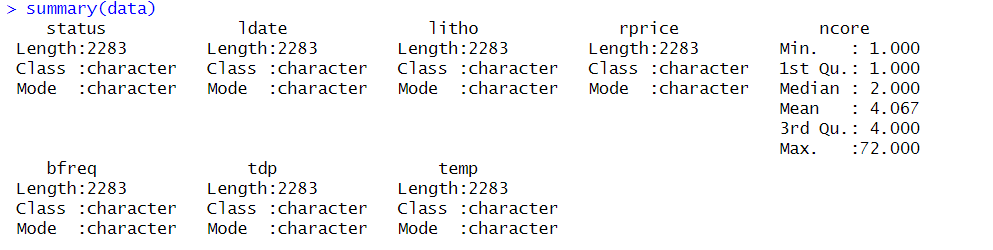
\includegraphics[max width=0.7\linewidth]{graphics/new_graphics/New data/summary-of-data-before.png}
    \caption{Summary of data before cleaning.}
\end{figure}

\subsection{Checking missing value and data cleaning}
\label{subsection:data_cleaning}

After choosing the approriate attributes, we now have the subset of the original raw dataset. 
However, since the values vary in types (such as string, non-standard year-quarter format and numeric-string),
we might want transform them into reproducible types, so that the analysis later on is easier, homogeneous and accurate.

Note that this cleaning process \textbf{does not} remove the \mintinline{R}{NA} values, unless necessary. The reason is that, 
in one instance, there might be important values that should not be eliminated. Under different scopes of study, we can not treat 
instances with \mintinline{R}{NA} as an invalid datum for all scopes. In later sections, when we focus on a specific pattern of the data, only by then
that the data will have a tailored \mintinline{R}{NA} cleaning, and we will not, by chance, loose any important instance.

This process took \verb|/rcode/cpu-short.csv| from the importing procedure above as an input, and produce \verb|/rcode/cpu-clean.csv| as
an output.

\begin{figure}[H]
    \centering
    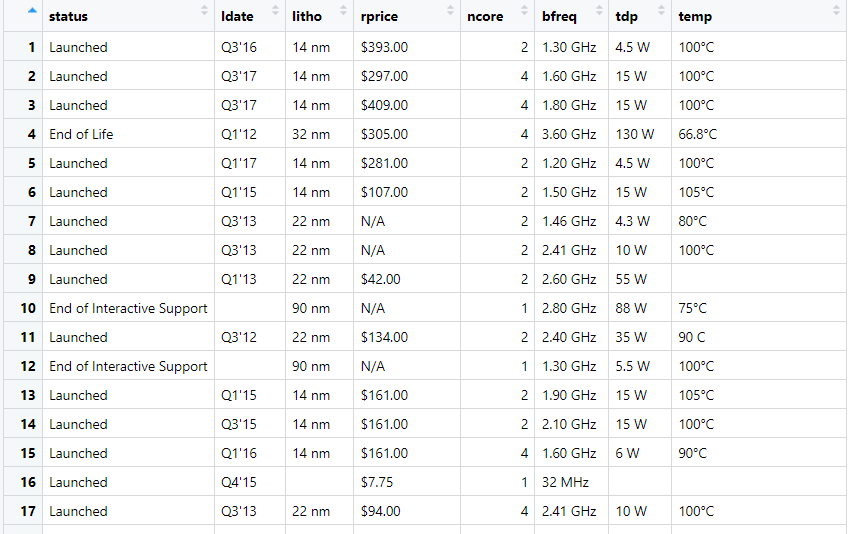
\includegraphics[max width=0.9\linewidth]{graphics/new_graphics/New data/Data-before.png}
    \caption{Data before cleaning.}
\end{figure}

\verb|market| and \verb|status| are left unchanged, since the values are straightforward. The remaining attributes (columns) are processed as followed:

\subsubsection*{Launch dates (ldate)}

\begin{code}{R}
data[,"ldate"] <- ( as.yearqtr(data[,"ldate"], format = "Q%q'%y"))
\end{code}

Our goal is to transform raw, non-standard year-quarter into \verb|zoo|'s standards. 
The function \mintinline{R}{as.yearqtr} takes a column and a format string as parameters. The format string is represented 
as: \mintinline{R}{"Q%q'%y"}, in which two flags \mintinline{R}{"%q"}, \mintinline{R}{"%y"} stands for quarter and year, respectively.
The format string hints the function to know the positions of quarter and year in our raw string.

\subsubsection*{Lithography (litho)}

\begin{code}{R}
data[,"litho"] <- as.numeric(gsub(" nm", "", data[,"litho"]))
\end{code}

Our goal is to cut out \verb|"nm"|, since every entry is recorded in nanometers anyway. In this code, \verb|gsub| substitutes 
the pattern \verb|" nm"| to \verb|""|. Notice that the pattern are regular expressions, and would be used intensively during 
this cleaning process.
% deprecated
\subsubsection*{Recommended Customer Price (rprice)}

\begin{code}{R}
data[,"rprice"] <- gsub("(^\\$(\\d)+.(\\d)+ - )", "", data[,"rprice"])
data$rprice <- ifelse(data$rprice == "N/A", NA, data$rprice)
data$rprice <- as.numeric(gsub('\\$|,', '', data$rprice))
\end{code}

Some \verb|rprice| values have ranges instead of sole numbers. We want to cut out uneccesary characters and only keep the largest price.
After that, we eliminate \verb|$| symbol from the string, as well as cast the string to numeric type.

\subsubsection*{Base frequency (bfreq)}

\begin{code}{R}
data[,"bfreq"] <- as.numeric(gsub("( GHz)|( MHz)", "", data[,"bfreq"]))
data<- data[!is.na(data$bfreq), ]
data$bfreq[data$bfreq > 10] <- data$bfreq[data$bfreq > 10]*0.001
\end{code}

Our goal is to cut out \verb|"GHz"| and \verb|"MHz"| from the string, and convert all \verb|"MHz"| values into \verb|"GHz"|. Heuristically,
we observed that any value greater than 10 must be \verb|MHz|, so we can transform every value like that will be multiply by 0.001 to get 
the according \verb|MHz| value.

\subsubsection*{Thermal design power (TDP)}
Same as for the \verb|litho| our goal is to simply also cut out W from the observation and change it to numeric type.

\begin{code}{R}
data[,"tdp"] <- as.numeric(gsub(" W", "", data[,"tdp"]))    
\end{code}

\subsubsection*{Temperature (temp)}

\begin{code}{R}
data[,"temp"] <- (gsub("[^0-9.\\-]+", ",", data[,"temp"]))
for (i in seq_along(data[["temp"]])) {
    temp_values <- strsplit(data[i, "temp"], ",") 
    temp_values <- unlist(lapply(temp_values, as.numeric))
    max_value <- max(temp_values, na.rm = TRUE)
    if (is.infinite(max_value)) {
        max_value <- NA
    }
    data[i, "temp"] <- max_value
}
export(data, "cpu-clean.csv")
\end{code}

Our goal is to only match the numeric values, then, take the maximum among those. The approach to processing the complicated strings in \verb|temp| is described as follows:
\begin{itemize}
    \item First, we attempt to match every decimal numbers possible, including the irrelevant number. The rest are replaced with commas \verb|","|.
    The result of this process will create a string of numbers separated by commas. By doing this, the numbers are well isolated for our purpose.

    \item Second, we split these numbers and form a vector of them. This can be done through \mintinline{R}{strsplit} function. Notice that our numbers
    are still in string format.

    \item Third, we cast all these strings to numeric and push them into a vector of values using \mintinline{R}{unlist} and \mintinline{R}{lapply}
    
    \item Fourth, we find the maximum among all these values. Invalid numbers will automatically become \(-\infty\), and will be further treated as \mintinline{R}{NA}.
    
    \item Notice that, we must loop through each row of the list to accomplish the above procedure.
\end{itemize}

Finally, the program produces \verb|cpu-clean.csv| as a cleaned data, ready for further exploitation in the later sections. In addition, \hyperlink{Listing 3}{\textit{\textcolor{blue}{Listing 3}}} and \hyperlink{Listing 4}{\textit{\textcolor{blue}{Listing 4}}} help us to identify the number of \mintinline{R}{NA} and \textbf{negative numbers}. Since there is no  \textbf{negative number} in our data, we skip the processing-with-negative-numbers process.

\begin{figure}[H]
    \centering
    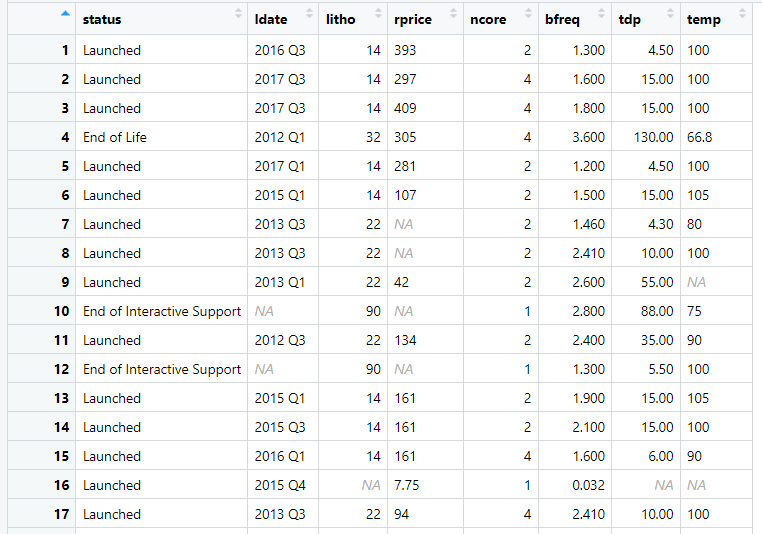
\includegraphics[max width=0.6\linewidth]{graphics/new_graphics/New data/Data-after.png}
    \caption{Data after cleaning.}
\end{figure}
\begin{code}{R}
    summary(data) ## Data summary after cleaning
    data$status<-as.factor(data$status)
    data$ldate<-as.factor(data$ldate)
    data$rprice<-as.factor(data$rprice)
    data$ncore<-as.factor(data$ncore)
    data$ncore<-as.factor(data$litho)
    ##Data summary by xtabs    
    xtabs(~status,data=data)
    xtabs(~ldate,data=data)
    xtabs(~litho,data=data)
    xtabs(~rprice,data=data)
    xtabs(~ncore,data=data)
    xtabs(~bfreq,data=data)
    xtabs(~tdp,data=data)
    xtabs(~temp,data=data)
\end{code}
\begin{figure}[H]
    \centering
    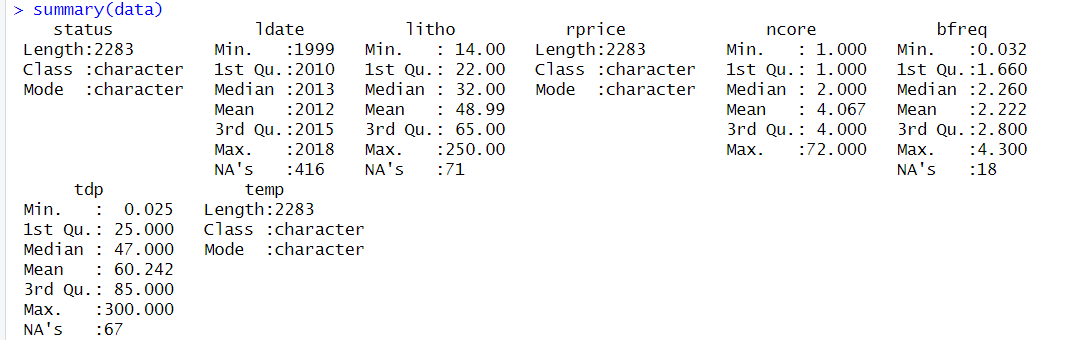
\includegraphics[max width=0.7\linewidth]{graphics/new_graphics/New data/summary-of-data-after.png}
    \caption{Data summary after cleaning.}
\end{figure}
\begin{figure}[!h]
\centering
    \begin{subfigure}[b]{0.49\textwidth}
        \centering
        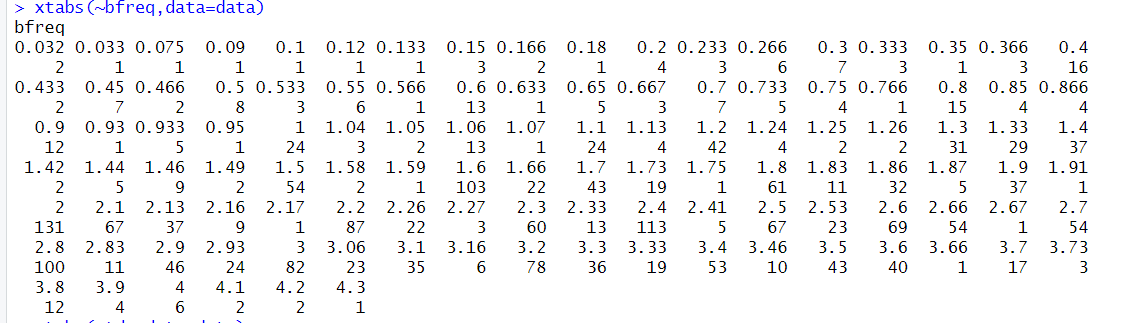
\includegraphics[width=\linewidth]{graphics/new_graphics/Xtabs/xtabs-bfreq.png}
        \caption{Summary of Base frequency.}
    \end{subfigure}
    \begin{subfigure}[b]{0.49\textwidth}
        \centering
        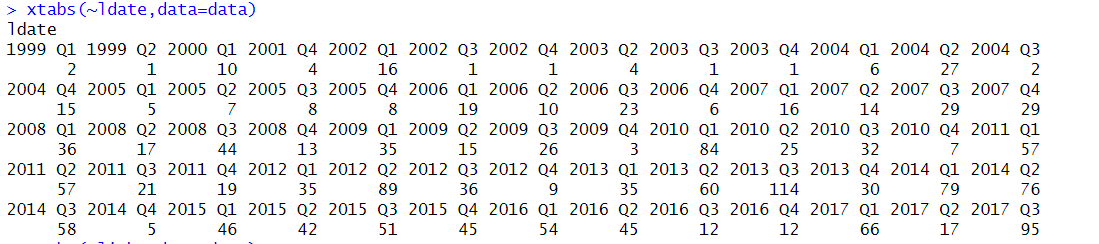
\includegraphics[width=\linewidth]{graphics/new_graphics/Xtabs/xtabs-ldate.png}
        \caption{Summary of Launch date.}
    \end{subfigure}
    \hfill
    \begin{subfigure}[b]{0.49\textwidth}
        \centering
        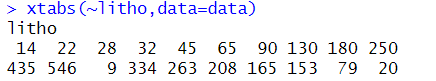
\includegraphics[width=\linewidth]{graphics/new_graphics/Xtabs/xtabs-litho.png}
        \caption{Summary of Lithography.}
    \end{subfigure}

    \begin{subfigure}[b]{0.49\textwidth}
        \centering
        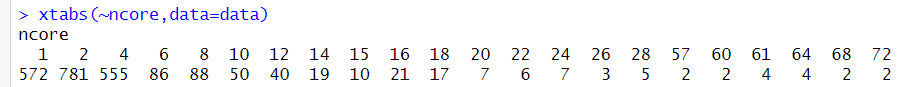
\includegraphics[width=\linewidth,height=0.4\linewidth]{graphics/new_graphics/Xtabs/xtabs-ncore.png}
        \caption{Summary of Number of Core.}
    \end{subfigure}
    \hfill
     \begin{subfigure}[b]{0.49\textwidth}
        \centering
        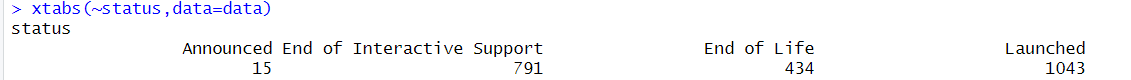
\includegraphics[width=\linewidth,height=0.4\linewidth]{graphics/new_graphics/Xtabs/xtabs-status.png}
        \caption{Summary of Status.}
    \end{subfigure}
    \begin{subfigure}[b]{0.49\textwidth}
        \centering
        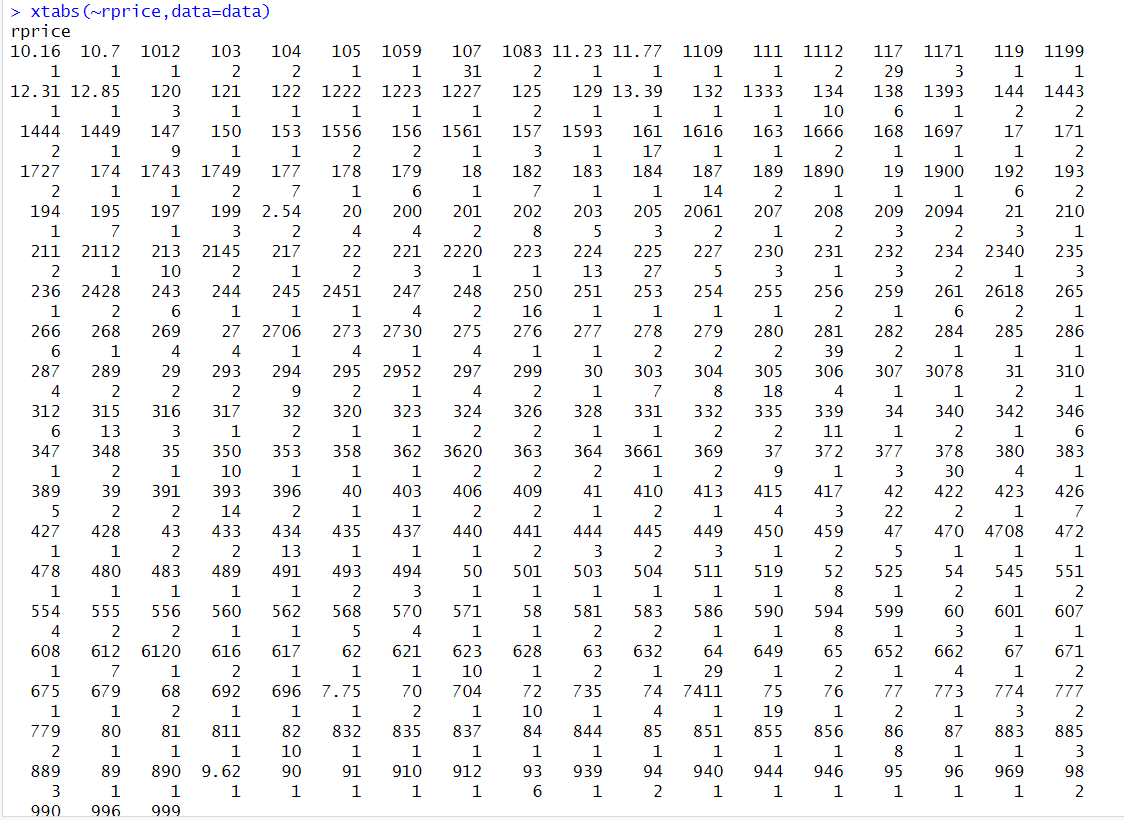
\includegraphics[width=\linewidth]{graphics/new_graphics/Xtabs/xtabs-rprice.png}
        \caption{Summary of Recommend Price.}
    \end{subfigure}
   \hfill
    \begin{subfigure}[b]{0.49\textwidth}
        \centering
        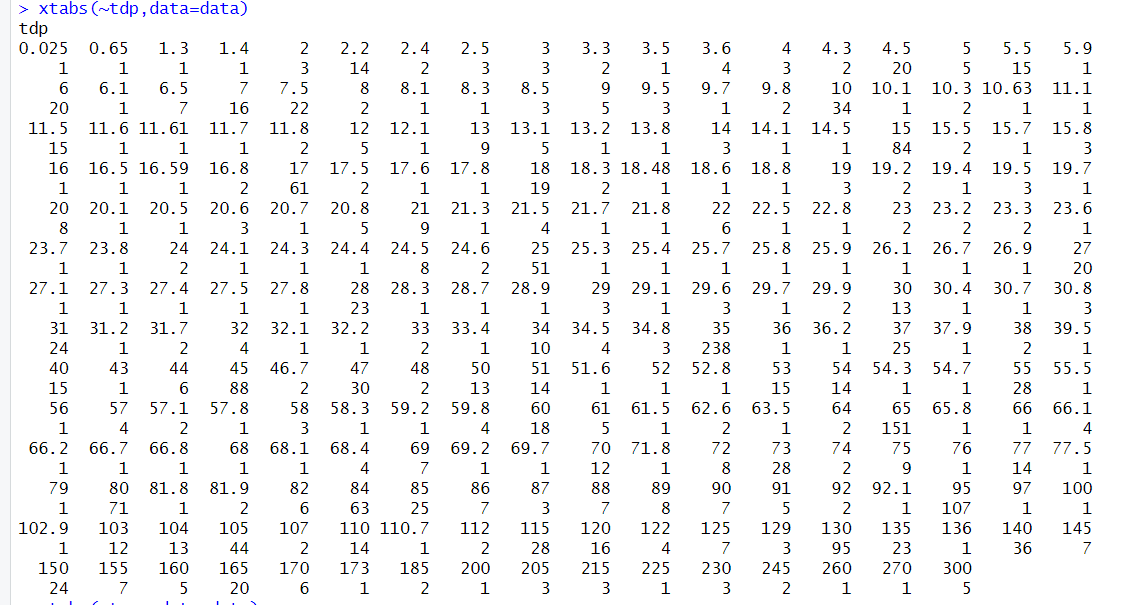
\includegraphics[width=\linewidth]{graphics/new_graphics/Xtabs/xtabs-tdp.png}
        \caption{Summary of Thermal design power.}
    \end{subfigure}
    \begin{subfigure}[b]{0.49\textwidth}
        \centering
        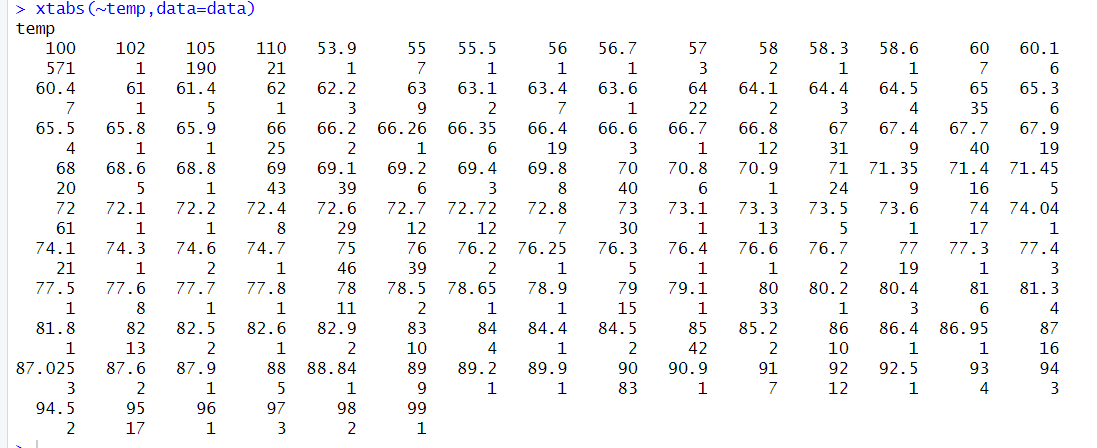
\includegraphics[width=\linewidth]{graphics/new_graphics/Xtabs/xtabs-temp.png}
        \caption{Summary of Temperature.}
    \end{subfigure}
    \caption{Summary of data by using command xtabs.}
\end{figure}
We remove the \mintinline{R}{NAs} rows from the data set, note that only the
\mintinline{R}{NAs} associated with specific columns are removed, the reason not to remove all is described in \textbf{Section \ref{subsection:data_cleaning}}.

\begin{code}{R}
    data <- data[!is.na(data$tdp), ]
    data <- data[!is.na(data$bfreq), ]
    data <- data[!is.na(data$litho), ]
    data <- data[!is.na(data$ncore), ]
    data <- data[!is.na(data$temp), ]
\end{code}

% END OF DATA CLEANING
%
%   Descriptive statistics
%       - Plots...
%   
\section{Descriptive statistics}
\label{section:discriptive_stats}

\begin{figure}[H]
    \centering
    \begin{subfigure}[b]{0.49\textwidth}
        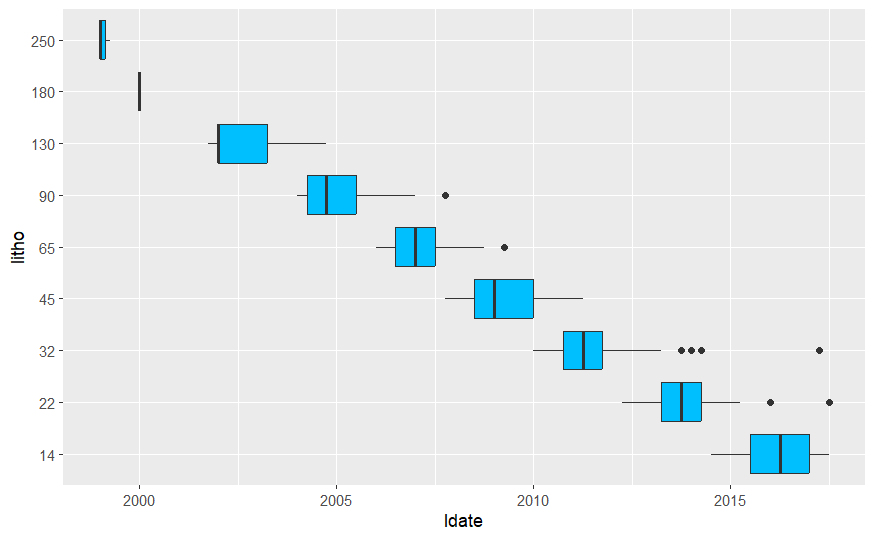
\includegraphics[width=\textwidth]{graphics/boxplot_litho_ldate.png}
        \caption{Box plots and Summary of Lithography}
        \label{fig:box_litho}
    \end{subfigure}
    \hfill
    \begin{subfigure}[b]{0.49\textwidth}
        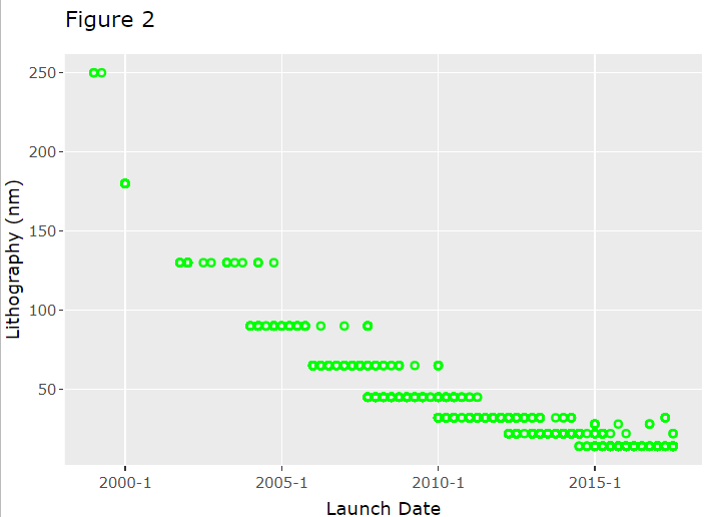
\includegraphics[width=\textwidth]{graphics/new_graphics/Fig2.png}
        \caption{Plot of lithography over time.}
        \label{fig:scatter_litho}
    \end{subfigure}
    \caption{Lithography plots}
    \label{litho-ldate}
\end{figure}

\begin{code}{R}
ggplot(data, aes(x = ldate, y = litho)) +
  geom_boxplot(fill="deepskyblue")
ggplot(data, aes(x = ldate, y = litho)) +
    geom_point(shape = 1,color = "blue") +
    labs(x = "Launch Date", y = "Lithography (nm)")
\end{code}

The scatter plot of \textit{Lithography} \textbf{[Figure \ref{litho-ldate}]} 
shows that it is getting smaller over time, and is categorized into specific time intervals.
\textit{Lithography} spans the distribution over an interval of time which make it more powerful than \textit{Launch date}. In our
models, we always use \textit{Lithography} instead of \textit{Launch date}. Which we will be proving later in \ref{Litho era}.









\begin{figure}[H]
    \centering
    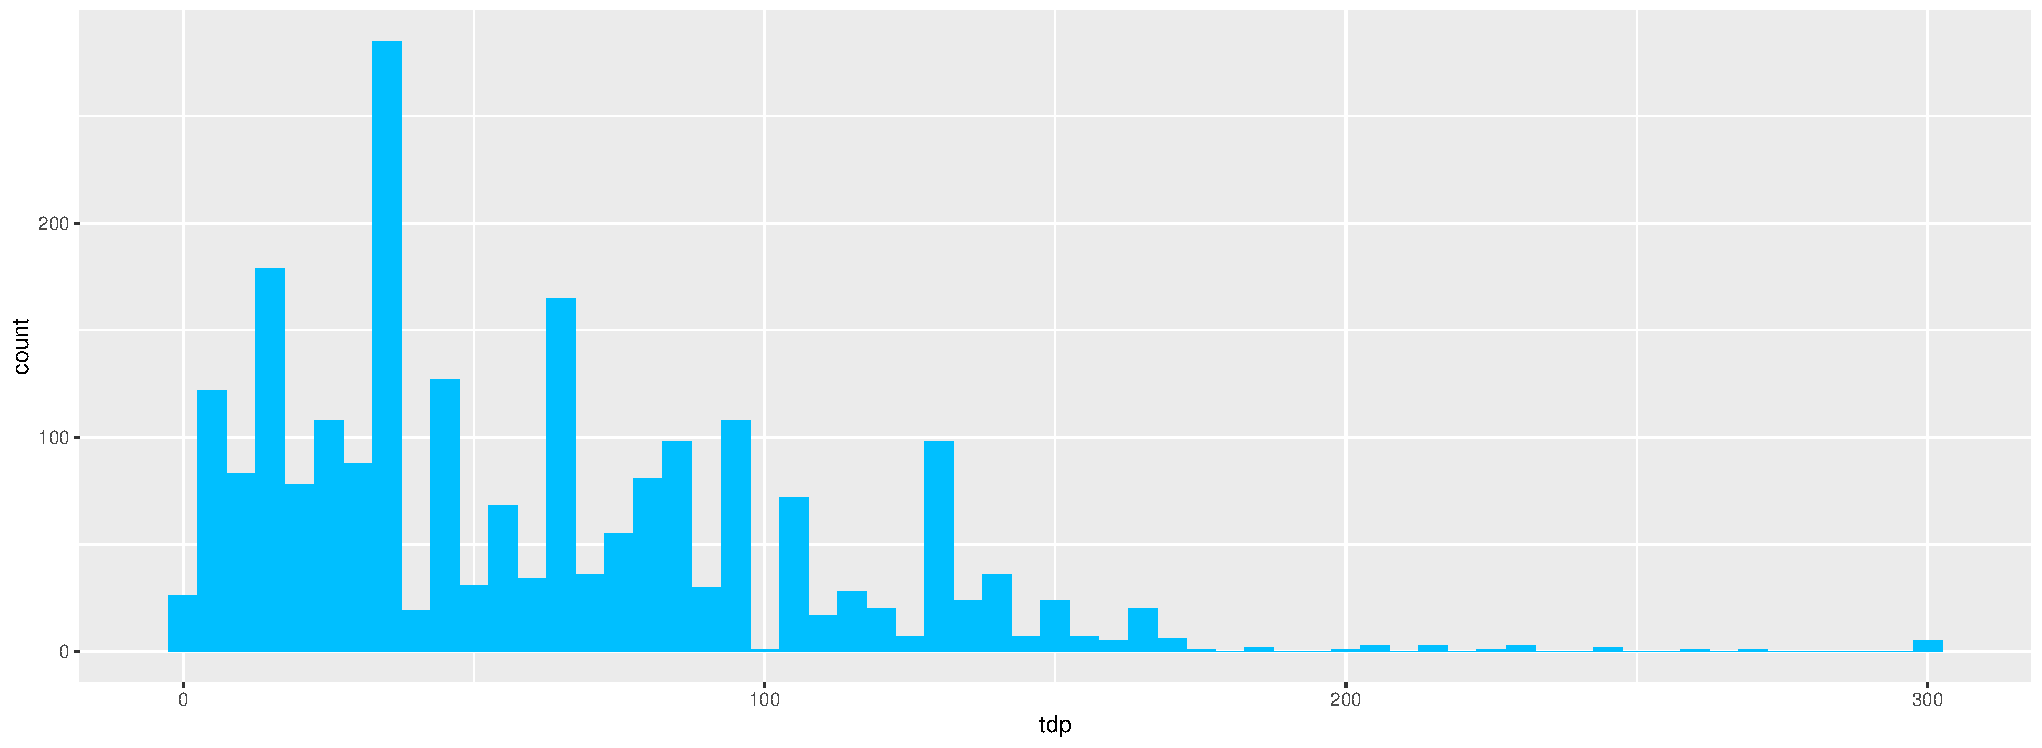
\includegraphics[width=0.75\textwidth]{./graphics/hist_tdp.pdf}
    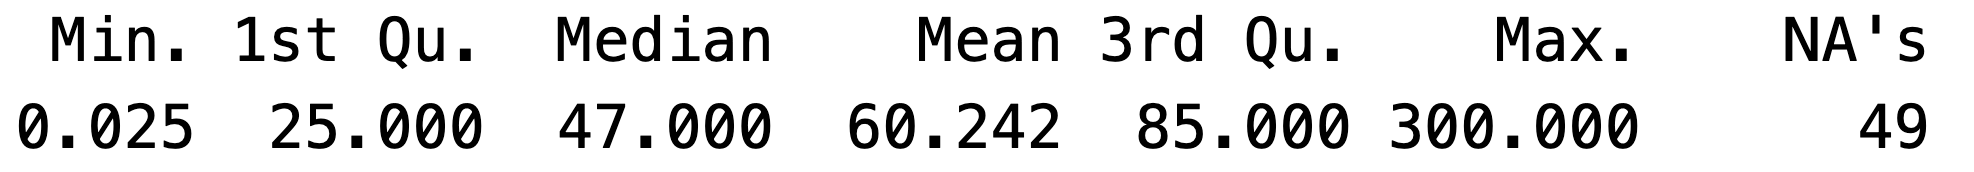
\includegraphics[width=0.6\textwidth]{./graphics/sum_tdp.png}
    \caption{Histogram and Summary of Thermal Design Power}
    \label{fig:hist_tdp}
\end{figure}

\begin{code}{R}
ggplot(data, aes(x = tdp)) +
  geom_histogram(binwidth = 5, fill = "deepskyblue")
summary(data$tdp)
\end{code}

\textbf{[Figure \ref{fig:hist_tdp}]} The occurrences of values $\ge 150$W are very rare, 
so they could be treated as outliers in further analysis.









\begin{figure}[!h]
    \centering
    
    \begin{subfigure}[b]{0.49\textwidth}
        \centering
        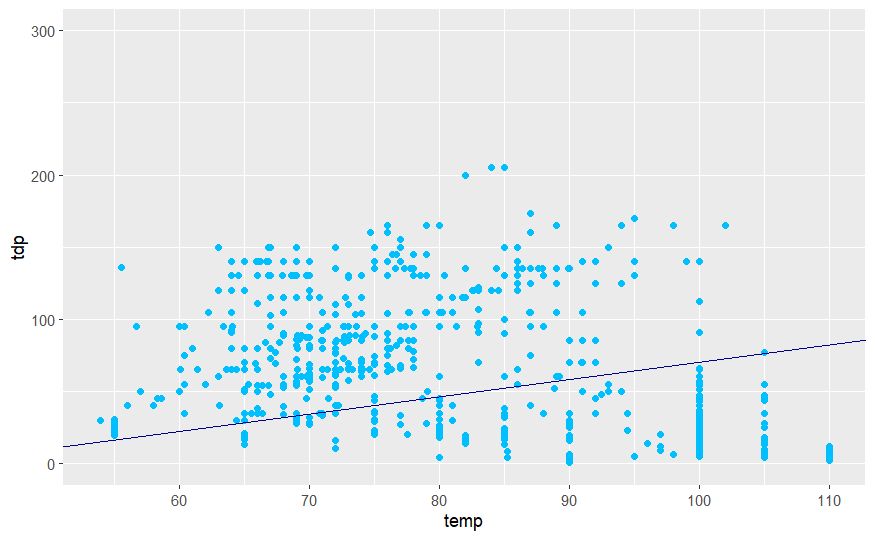
\includegraphics[width=\textwidth]{./graphics/scatter_tdp_temp.png}
        \caption{Different trends of TDP on different ranges of temperature}
        \label{fig:tdp_analysis_temp}
    \end{subfigure}
    \begin{subfigure}[b]{0.49\textwidth}
        \centering
        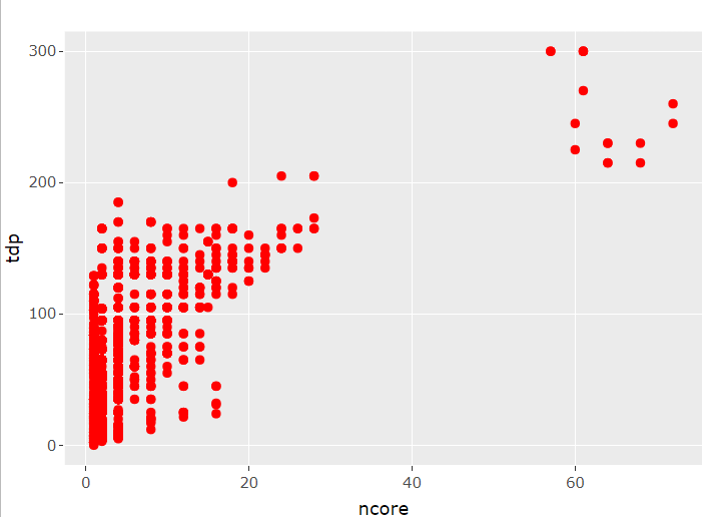
\includegraphics[width=\textwidth]{graphics/new_graphics/Fig5.png}
        \caption{Increasing trend of no. cores and TDP}
        \label{fig:tdp_analysis_ncore}
    \end{subfigure}
\end{figure}






\begin{figure}[!h]
\centering
    \begin{subfigure}[b]{0.49\textwidth}
        \centering
        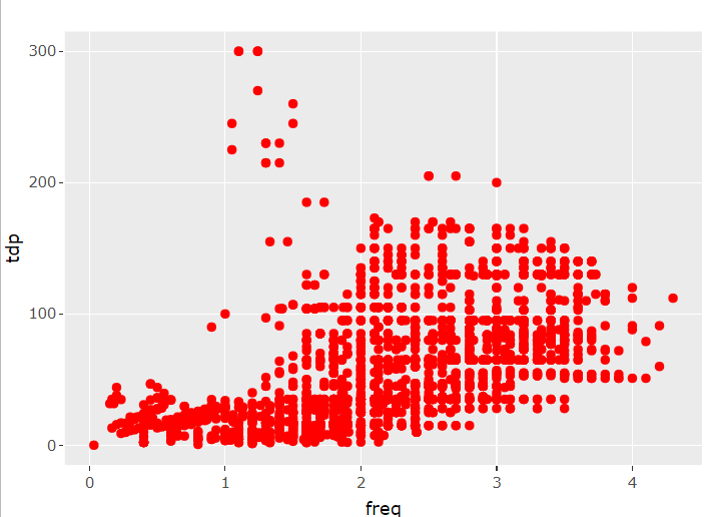
\includegraphics[width=\textwidth]{graphics/new_graphics/Fig4.png}
        \caption{Increasing trend of Base frequency and TDP}
        \label{fig:tdp_analysis_bfreq}
    \end{subfigure}
    \begin{subfigure}[b]{0.49\textwidth}
        \centering
        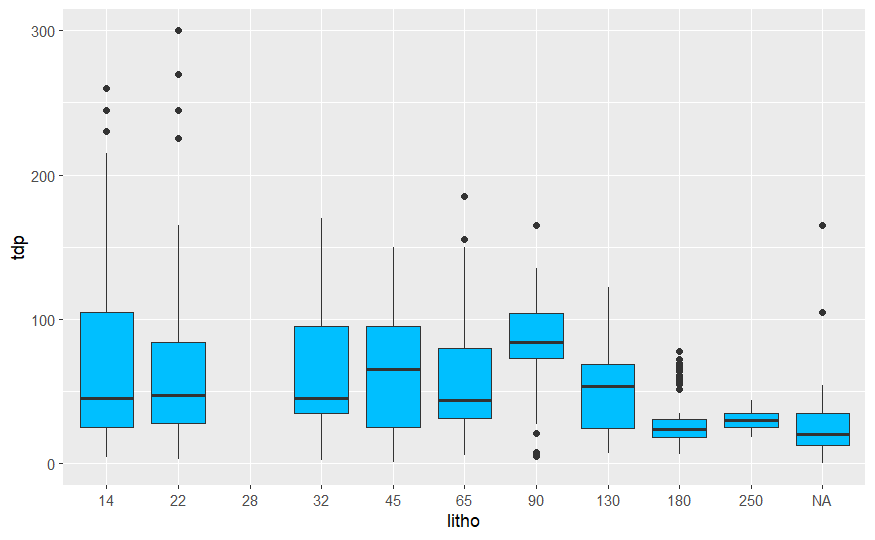
\includegraphics[width=\textwidth]{graphics/boxplot_tdp_litho.png}
        \caption{TDP within different Lithography}
        \label{fig:tdp_analysis_litho}
    \end{subfigure}
    \hfill
    \caption{The relationship visualizations between TDP and other factors}
    \label{fig:tdp_analysis}
\end{figure}

\begin{code}{R}
ggplot(data, aes(x = tdp)) +
  ggplot(data, aes(x = temp, y = tdp)) +
  geom_point(color = "deepskyblue", ) +
  geom_abline(mapping = aes(intercept = -50, slope = 1.2), color = "darkblue")
ggplot(data, aes(x = ncore, y = tdp)) +
  geom_point(color = "deepskyblue")
ggplot(data, aes(x = bfreq, y = tdp)) +
  geom_point(color = "deepskyblue")
ggplot(data, aes(x = litho, y = tdp)) +
  geom_boxplot(fill = "deepskyblue")
\end{code}

From the above visualizations, we could make a few comments from these relationships, which motivates us to use certain Regression models:
\begin{itemize}
    \item \textbf{[Figure \ref{fig:tdp_analysis_ncore}]} \verb|tdp ~ ncore| : As \verb|ncore| increases, \verb|TDP| also increases. This motivates us to use 
    a Linear regression model. However, we also observe that, there are distinctive "clusters" on different ranges. Maybe a decision-based model, like Random Forrest,
    is better.
    
    \item \textbf{[Figure \ref{fig:tdp_analysis_bfreq}]} \verb|tdp ~ bfreq| : The data for this relationship is quite variant. However, the dominant trend is still linearly increasing,
    using Linear regression can be reliable.
    
    \item \textbf{[Figure \ref{fig:tdp_analysis_litho}]} \verb|tdp ~ litho| : There is no clear upward and downward trend. Instead, \verb|TDP| is converging and gets more and more stable over time. 
    
  %  \item \textbf{[Figure \ref{fig:tdp_analysis_temp}, \ref{fig:tdp_analysis_market}]} \verb|tdp ~ temp| and \verb|tdp ~ market| : There are two different trends happening: 
%    above the reference line is increasing trend, while below is decreasing trend. In fact, we have a feeling that these two trends come from 
%    different market segments \verb|type=(Desktop + Server)| \verb|(Mobile + Embedded)|, so we would plot them out to verify:

%        \begin{code}{R}
%data$type <- ifelse(data$market == 'Server' | %data$market == 'Desktop', "Computers", "Devices")
%data$type <- as.factor(data$type)

%ggplot(data, aes(x = type, y = tdp)) +
%    geom_boxplot(fill = "deepskyblue")
            
%ggplot(data, aes(x = temp, y = tdp)) +
%    geom_point(color = "deepskyblue", ) +
%facet_wrap(~data$type)
%        \end{code}

%        \begin{figure}[H]
%            \centering
 %           \begin{subfigure}[]{0.4\textwidth}
 %               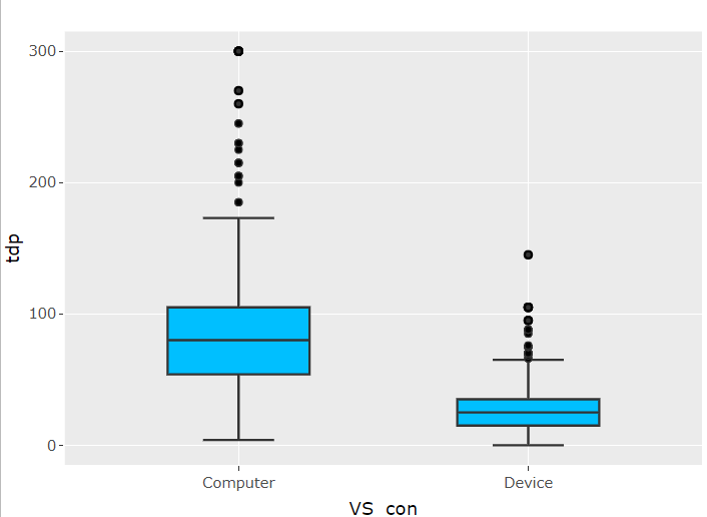
\includegraphics[width=\textwidth]{graphics/new_graphics/Fig7.png}
 %               \caption{TDP between Types.}
 %           \end{subfigure}
 %           \begin{subfigure}[]{0.4\textwidth}
 %               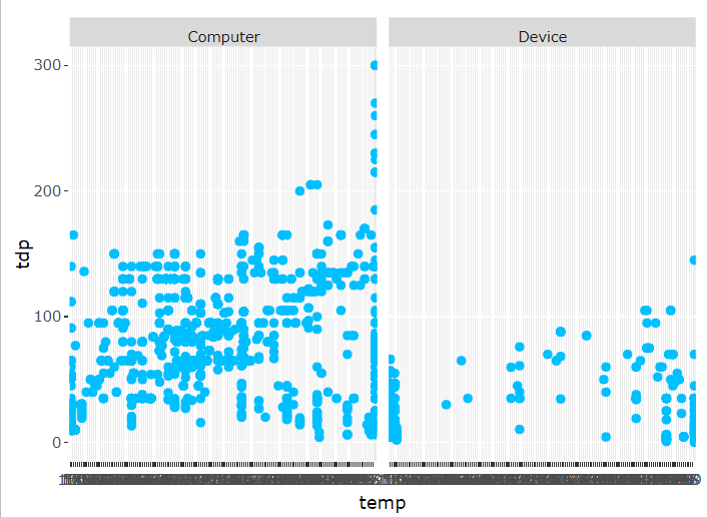
\includegraphics[width=\textwidth]{graphics/new_graphics/Fig8.png}
 %               \caption{TDP in different Market segmentation}
 %           \end{subfigure}
 %       \end{figure}
        \end{itemize}
        
%Turns out, different trends belongs to different Market segments (\verb|type|). This could be helpful for us to classify the \verb|TDP| into different markets using Logistic regression.

%
%   Data Analysis
%       - ANOVA and Regression and stuff.
%   
\section{Inferential statistics}
\label{section:infer_stats}

As stated in our Report's title, the main focus of the analysis will be \textit{Thermal Design Power} and the affect of
other attributes (variables) on this dependent variable.

\textit{Thermal Design Power} \verb|TDP| is an interesting characteristic that comes with the CPU. Theoretically, this is the
maximum amount of heat that can be released by its cooling system, which should never be exceeded. This characteristic somehow
represents the heat barrier of a processor, and if its cooling system is designed to deal with almost all the heat it release,
\verb|TDP| roughly equates to its power consumption. The higher the \verb|TDP|, the better the CPU's cooling system, but also 
demonstrates the amount of energy consumption required to dissipate the heat.

The reason why we did not use \textit{Temperature} but instead \textit{Thermal Design Power} is that we want to find the amount of
energy needed to keep the CPU operational properly, not the temperature point that the CPU can work but be potentially damaged.

We would try to utilize some Regression models to predict its \verb|TDP| via other configurations (or determinants) such as
\textit{Thermal design power}, \textit{Number of cores}, \textit{Base frequency}, \textit{Temperature}, \textit{Lithography} and its \textit{Status}.
%\textit{Market} and its \textit{Status}.% Also, we will see if with the determined \verb|TDP|, we can classify the CPU, whether
%it belongs to mass computing devices (Server) or personal usage (Desktop and Mobile).



\subsection{Data preparation}

First, we load the cleaned data set from the cleaning process above.

\begin{code}{R}
pacman::p_load(
    rio,     # for imports & exports
    ggplot2, # for plots
    zoo,      # for year-quarter formats
    car     # for levent and shapiro
)
data <- import("cpu-clean.csv") # rio::import
\end{code} 

Refer to \textbf{[Figure 7]} and our statement previously, the occurrences of values $\ge 150$ is rare, we decided to
cut them out from our data set.
\begin{code}{R}
    data <- data[data$tdp < 150, ]
\end{code} 

Because we would make use of Regression models to capture the relationships, a Test Set and a Training Set must be present to perform 
cross-validation to test the fitness of the model, besides visualization method by drawing graphs and checking other coefficients. The original
data set is splitted into two smaller sets, training set and validated set (or test set). In detail, 80% data is used for training set while 20% 
is used for test set.

\begin{code}{R}
set.seed(123)

train_indices <- sample(1:nrow(data), nrow(data) * 0.8)
train <- data[train_indices, ]
test <- data[-train_indices, ]
\end{code}

\begin{itemize}
    \item To make a random generation homogeneous among all our tests, we specified a seed (123). Each time we run the cell, we would get
    consistent results of the split.
    \item \verb|sample()| helps us to take a sample from all the elements of our data set using without replacement. The return value of this function
    are the indices of 80% the data set, randomly chosen.
    \item After that, we use a simple indexing technique to assign to a training set and test set, accordingly.
\end{itemize}









\subsection{The relationships between TDP and other factors}
\subsubsection{Hypothesis testing}
\label{section:data_analysis_anova}

To explain further the statements we made above, we will assess the following assumptions by using several techniques such as 
hypothesis testing, ANOVA and computing the covariances.

The assumptions we are aiming to:
\begin{enumerate}
    \item Lithography as a CPU era.
    \item Thermal Design Power with respect to lithography.
    % \item Thermal Design Power with respect to Temperature.
\end{enumerate}



\subsubsection{Lithography as a CPU era.\label{Litho era}}

In this small section, we will demonstrate why \textbf{Lithography as a better representative than Launch date}. To do that, we start by looking at the confidence interval and the visualizations of Lithography over the years.

\begin{code}{R}
    data$litho <- as.factor(data$litho)
    retval <- data.frame(NA, NA, NA, NA)
    names(retval)<-c("5% quantile","95% quantile", "STD Mean", "Confidence Interval")
    for (lit in levels(data$litho))
    {
          quants <- quantile(
            data[data$litho == lit, ]$ldate,
            na.rm = T,
            probs = c(0.05,0.95)
          )
          dates <- data[data$litho == lit, ]$ldate
          new_row <- data.frame(quants[1], quants[2], mean(sd(dates, na.rm=TRUE), na.rm=TRUE),quants[2]-quants[1])
          names(new_row)<-c("5% quantile","95% quantile", "STD Mean", "Confidence Interval")
          retval <- rbind(retval, new_row)
          rm(dates)
    }
    rownames(retval) <- c("NULL", levels(data$litho))
    retval <- retval[-1,]
    print(retval)
\end{code}
\begin{figure}[H]
    \centering
    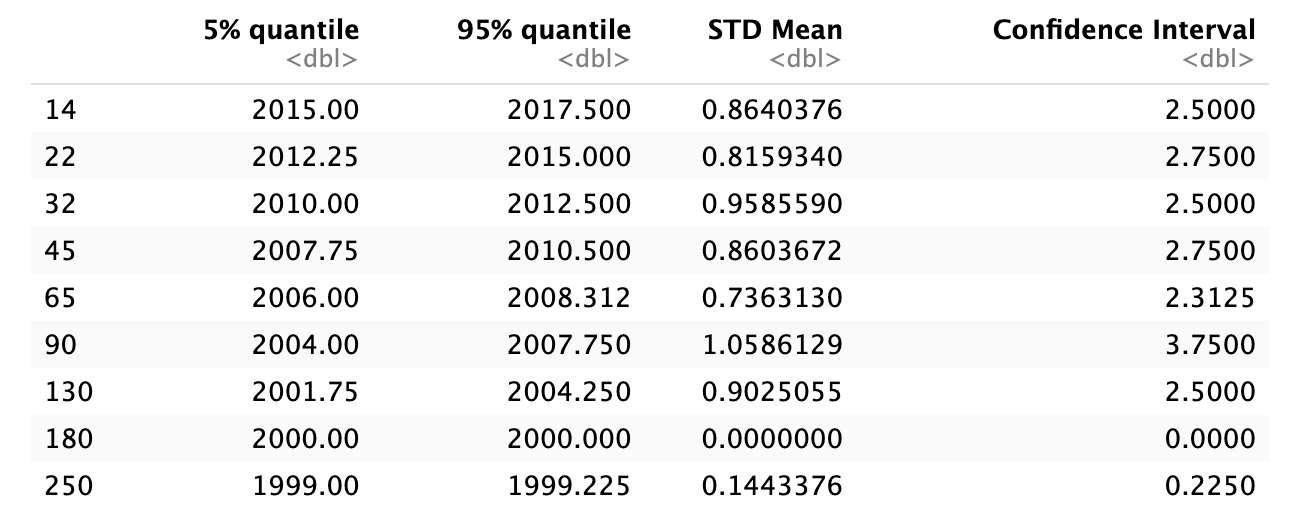
\includegraphics[width=0.5\textwidth]{./graphics/confint_litho.png}
    \caption{Summary of Confidence Interval of Lithography over the years}
\end{figure}

Looking at the Mean of Standard Deviation (\verb|STD Mean|), these \textit{means are pretty stable}, and the \verb|Confidence Interval| column tells us that
most of the era of CPU design \textit{spans for about two and a half years}, and these era are approximately mutually exclusive. This is its big advantage over
using Launch date only, because we can now consider a range of values and group different launch dates together wich possibly share the same characteristics. So,
everytime we wants to refer to a period of CPU, we always use Lithography.





\subsubsection{Thermal Design Power with respect to lithography.}







One more thing we want to emphasize is the \textbf{stability of TDP in recent eras}, and the fact that it is converging. We will do the ANOVA to test and see if there is a significant difference in the tdp between the lithography era.

We will have the null hypothesis:
$H_0$: the mean of the tdp in each type of lithography is the same.
$H_1$: there exists a pair of lithography type so that their mean is different.

From the Descriptive statistics, we can see that there are particularly few CPUs with lithography of 28 and 250, so we will remove them as well as all the row that has \mintinline{R}{NA} value
\begin{code}{R}
    # remove data with few count group ldate and remove NA
    data <- data[data$litho !=28,] 
    data <- data[data$litho !=250,] 

    data <- data[!is.na(data$tdp), ]
    data <- data[!is.na(data$litho), ]
\end{code}

We will create an ANOVA model.

\begin{code}{R}
    litho_anova_model<- aov(tdp ~ litho ,data = data)
\end{code}

Getting the result of the model.

\begin{code}{R}
    summary(litho_anova_model)
\end{code}

\begin{figure}[htbp]
    \centering
    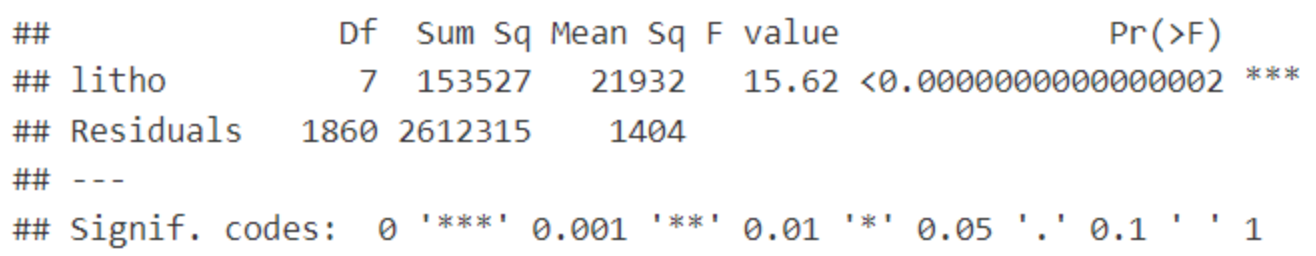
\includegraphics[width = 0.6\textwidth]{graphics/litho_anova_model.png}
\end{figure}

We can see that as the p-value < 0.05, we can reject the null hypothesis $H_0$ and accept the 
alternative hypothesis $H_1$ that there exists a pair of \verb|litho| type so that their \verb|TDP| mean is difference.

To satisfy the requirements of One-way ANOVA, we should check its assumptions on Normality and Homoscedasticity (homogeneous variance).

\begin{code}{R}
    qqPlot(residuals(litho_anova_model))
    shapiro.test(residuals(litho_anova_model))
    leveneTest(tdp ~ litho ,data = data)
\end{code}
\begin{itemize}
    \item We make a Q-Q Plot to explore its residuals.

    \item We perform a Shapiro-Wilk test of Normality:
    
        \qquad Null hypothesis $H_0$ : The residuals of the ANOVA model are normally distributed.

        \qquad Alternative hypothesis $H_1$ : The residuals of the ANOVA model is not normally distributed.

    \item We perform Levene's test to test for the equality of variances.
    
        \qquad Null hypothesis $H_0$ : The variance of \verb|TDP| between categorical \verb|litho| is equal.

        \qquad Alternative hypothesis $H_1$ : The variance between them is not equal.
\end{itemize}

\begin{figure}[H]
    \centering
    \begin{subfigure}[b]{0.35\textwidth}
        \centering
        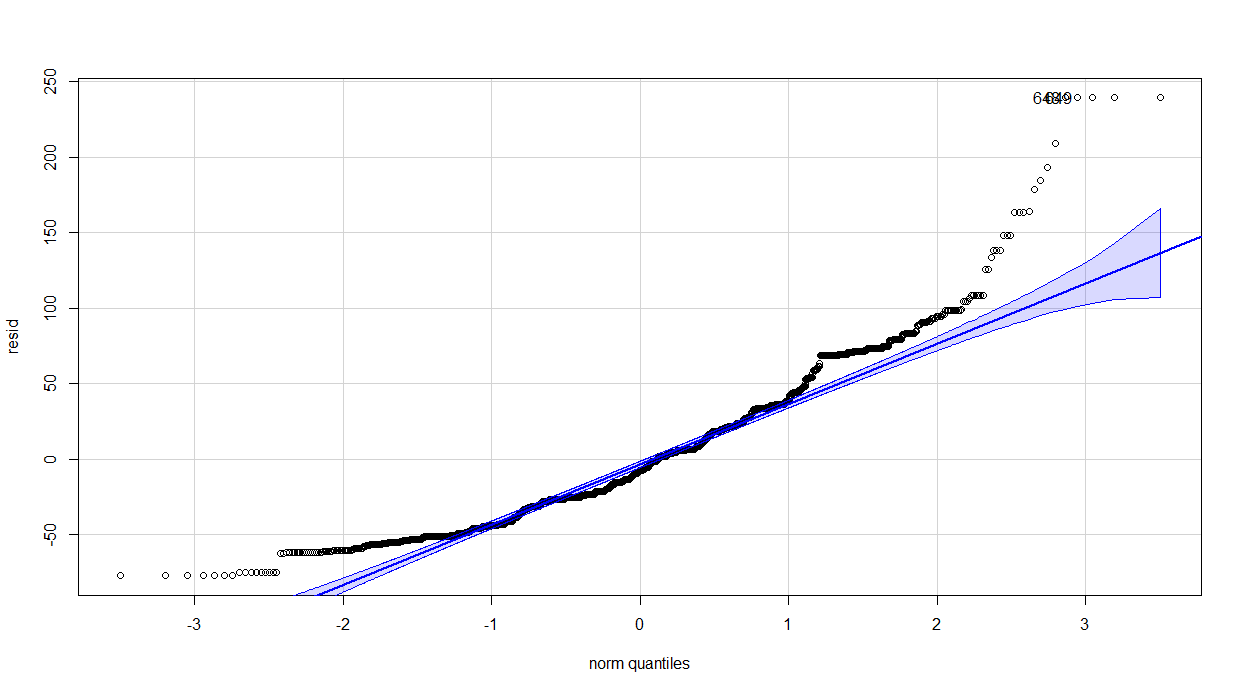
\includegraphics[width=\textwidth]{./graphics/QQplot_resid_litho.png}
        \caption{Q-Q Plot of the ANOVA model}
        \label{fig:anova_litho_shapiro_wilk}
    \end{subfigure}
    \begin{subfigure}[b]{0.6\textwidth}
        \centering
        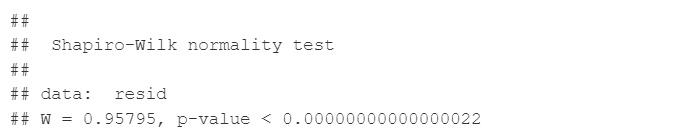
\includegraphics[width=\textwidth]{graphics/shapiro.png}
        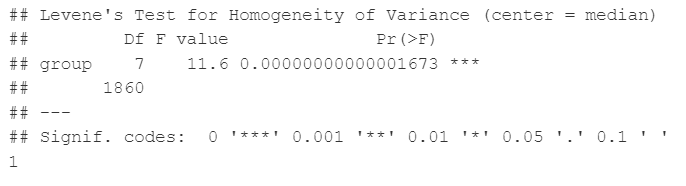
\includegraphics[width=\textwidth]{graphics/levent.png}
        \caption{Results of Shapiro-Wilk and Levene's Test}
        \label{fig:anova_litho_shapiro_wilk}
    \end{subfigure}
    \caption{Summary of the tests.}
\end{figure}

We can see that the normality and variance test both fail as their p-value is both less than 0.05 and the qqplot has a lot of point that deviate from the line, however, the ANOVA test are also resilient against the violation of the two assumptions\cite{tukey}. 

Finally we will analyse the result with a post hoc test to see which mean are different from each other. For this, we will use the TUKEY HSD test for ANOVA.

\begin{code}{R}
    Tukey <- TukeyHSD(litho_anova_model)
    plot(Tukey,las = 2)
\end{code}
\newpage

\begin{figure}[htbp]
    \centering
    % \begin{subfigure}[b]{0.47\textwidth}
    %     \centering
    %     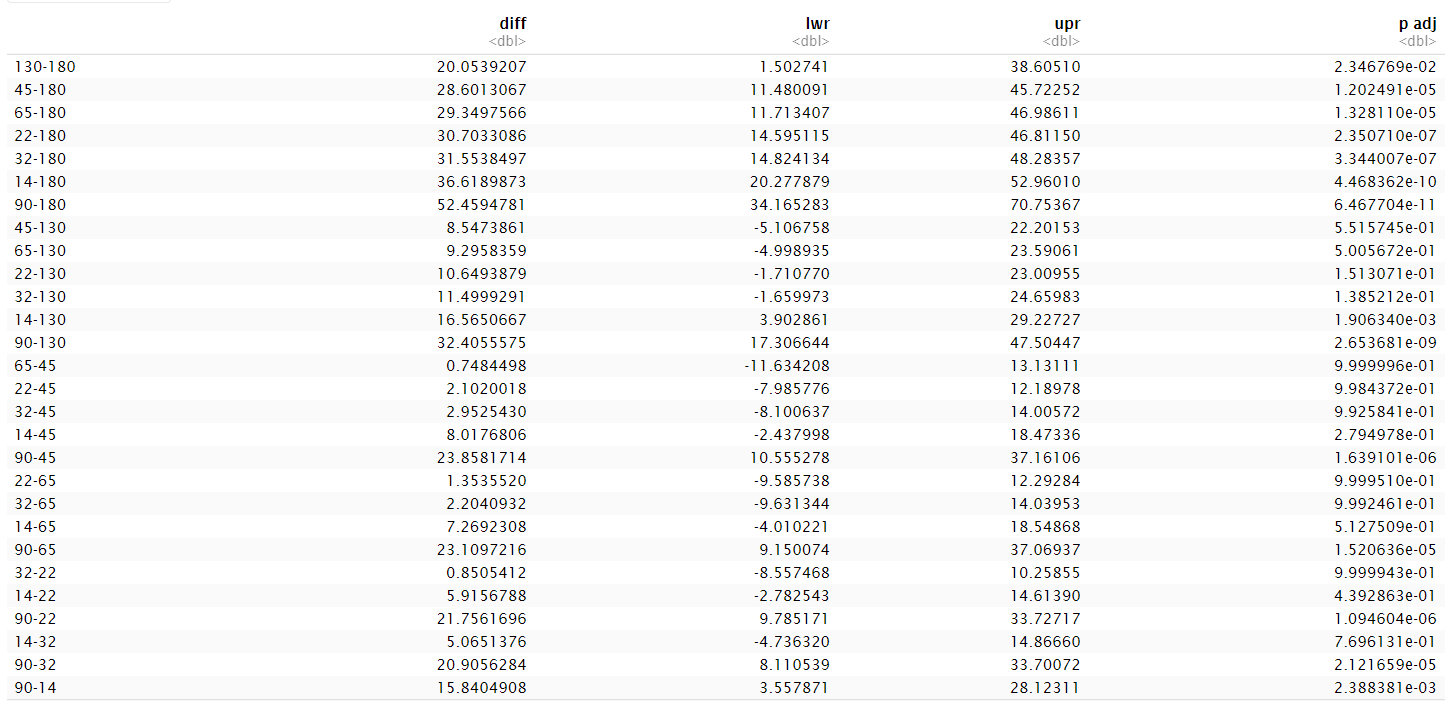
\includegraphics[width=\textwidth]{./graphics/TUKEY HSD.png}
    %     \caption{TUKEY HSD test result}
    %     \label{fig:TUKEY}
    % \end{subfigure}
    % \hfill

    \begin{subfigure}[b]{0.45\textwidth}
        \centering
        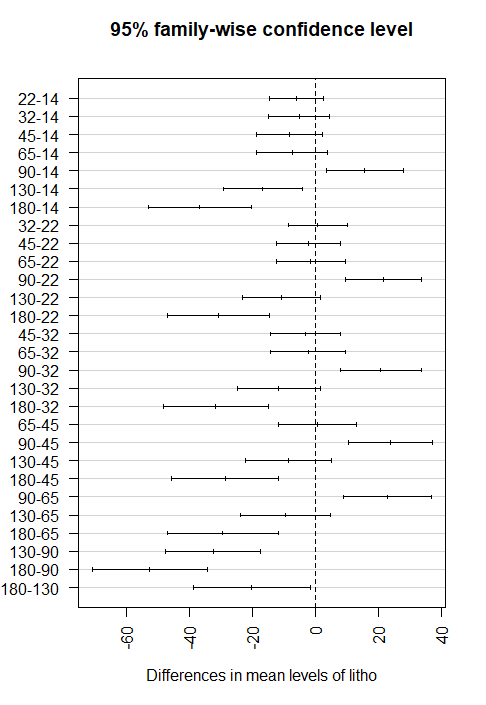
\includegraphics[width=\textwidth]{./graphics/TUKEY HSD confidence.png}
        \caption{TUKEY result plot}
        \label{fig:TUKEYconfidence}
    \end{subfigure}
    \caption{Summary of the post hoc tests.}
\end{figure}
% \begin{figure}
%     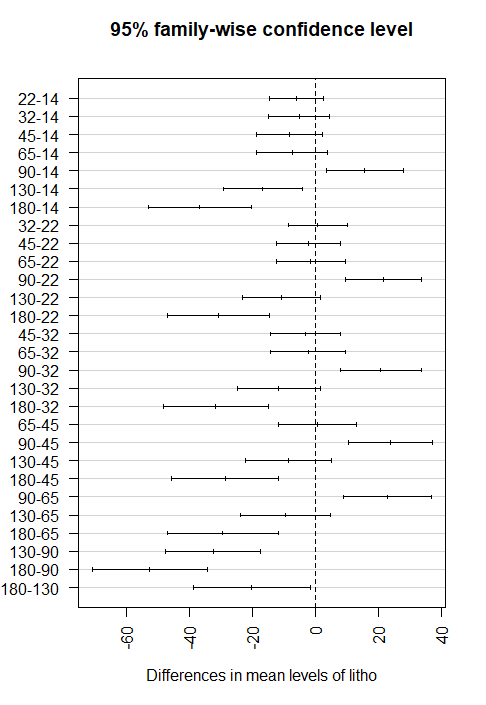
\includegraphics[width= 0.5\textwidth]{./graphics/TUKEY HSD confidence.png}
% \end{figure}
    

% \begin{figure}
%     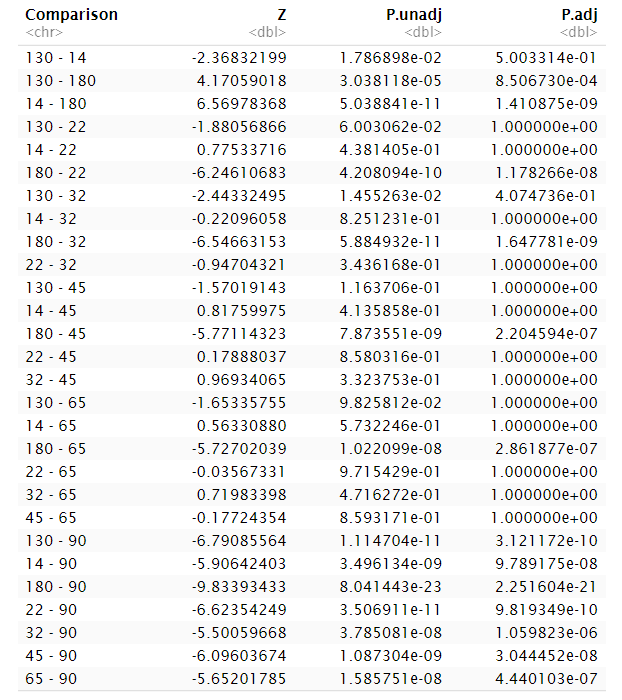
\includegraphics[width= 0.5\textwidth]{./graphics/dunntest.png}
% \end{figure}
We can interpret the result of our data as follow:
\begin{enumerate}
    \item There are a significant difference in \verb|tdp| 's mean and median between the CPU of bigger \verb|lithography|(180,130,90) and CPU of smaller \verb|lithography|(14,22,32,45,65)
    \item The CPU's \verb|lithography| from 14,22,32,45,65 have their mean being relatively the same.
    \item As \verb|lithography| also reflect \verb|release date|, as proven in \ref{Litho era} it also reflect the change in \verb|tdp| of CPU 's design over time.

    
\end{enumerate}

% The trend is clearly show that there are a significant difference in \verb|tdp| between cpu with bigger \verb|lithography|(180,130,90) and cpu of smaller \verb|lithography|(14,22,32,45,65). As have been proven in the  \ref{Litho era} i, we can see that the result also reflect the change in tdp over the year.




% \textbf{Thermal Design Power with respect to Temperature}

% Too really believe there are two trends of \verb|TDP| going on within \verb|temp|, we may want to split the \verb|temp| into
% two halves, one for \verb|temp < 85|, and one for \verb|temp >= 85|. Then we will compute the covariance too see if they are really
% different.

% \begin{itemize}
%     \item If the covariance is positive, the trend is likely to go upward,
%     \item If the covariance is negative, the trend is likely to go downward.
% \end{itemize}

% \begin{code}{R}
%     group1 <- data[data$temp < 85, ]
%     group2 <- data[data$temp >= 85, ]

%     cov(group1$tdp, group1$temp)
%     cov(group2$tdp, group2$temp)
% \end{code}

% The results are as follows:
% \begin{figure}[H]
%     \centering
%     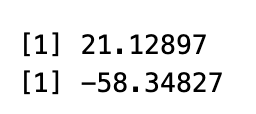
\includegraphics[width=0.3\textwidth]{./graphics/anova_temp_cov.png}
%     \caption{Q-Q plot of Temprature model}
%     \label{fig:anova_temp_cov}
% \end{figure}

% Two covariances are different from each other, meaning that there are two different trends going on.










\subsection{Regression analysis}
\noindent 

Base on checking the linearity of each column related to each other, in this section, we will conduct an investigation on the relationship between thermal design power with other features. There are many types of regression models, including simple linear regression, multiple linear regression, polynomial regression, logistic regression, and more. In this report, we will use certain model to test if there is any significant relationship between these figures.
\subsubsection{Predicting Multi-Linear Model}
\label{section:data_analysis_linear}

Since the scatter plot of the feature \textbf{thermal design power} (tdp) with other variable maybe related to Linear regression.
Now, first of all, we will build a linear regression model using \verb|lm()|.
\begin{code}{R}
# Build the model
model.lr <- lm(tdp ~ ncore + bfreq + temp, data = train)
# Summary of the model
summary(model.lr)
\end{code}

The \verb|summary()| command gives us an overview over some statistics of our model.
\begin{figure}[H]
    \centering
    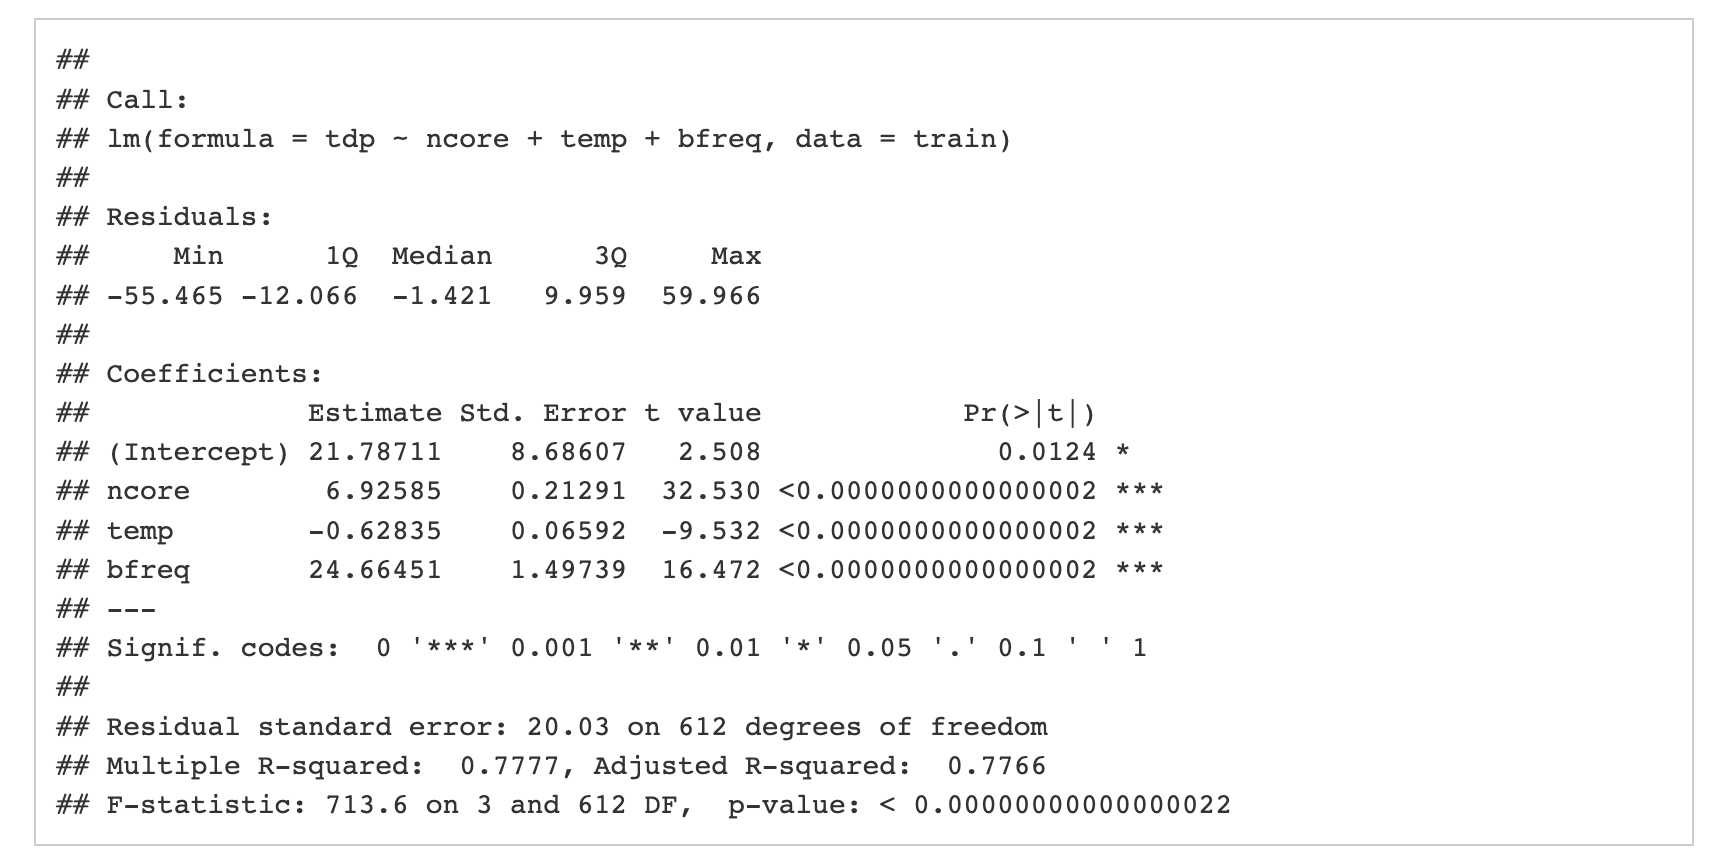
\includegraphics[width=0.8\textwidth]{graphics/linear_summary.png}
    \caption{Summary of linear model}
    \label{fig:30}
\end{figure}
We can observe that all of the variables have the p-value less than 0.05, therefore; all predictors that we have chosen is involved in the building process.

Now we must check for Multiple-Linear model assumption:
\begin{itemize}
    \item Residual Errors have a Mean Value of Zero.
    \item Residual Errors have Constant Variance.
    \item The errors are normally distributed.
\end{itemize}

\textbf{Testing for Residual Errors have a Mean Value of Zero:} We can check this assumption using the histogram of the residual:
\begin{code}{R}
ggplot(model.lr, aes(x = resid(model.lr))) +
  geom_histogram(binwidth = 2, fill = "deepskyblue") # histogram of residuals
\end{code}
\begin{figure}[H]
    \centering
    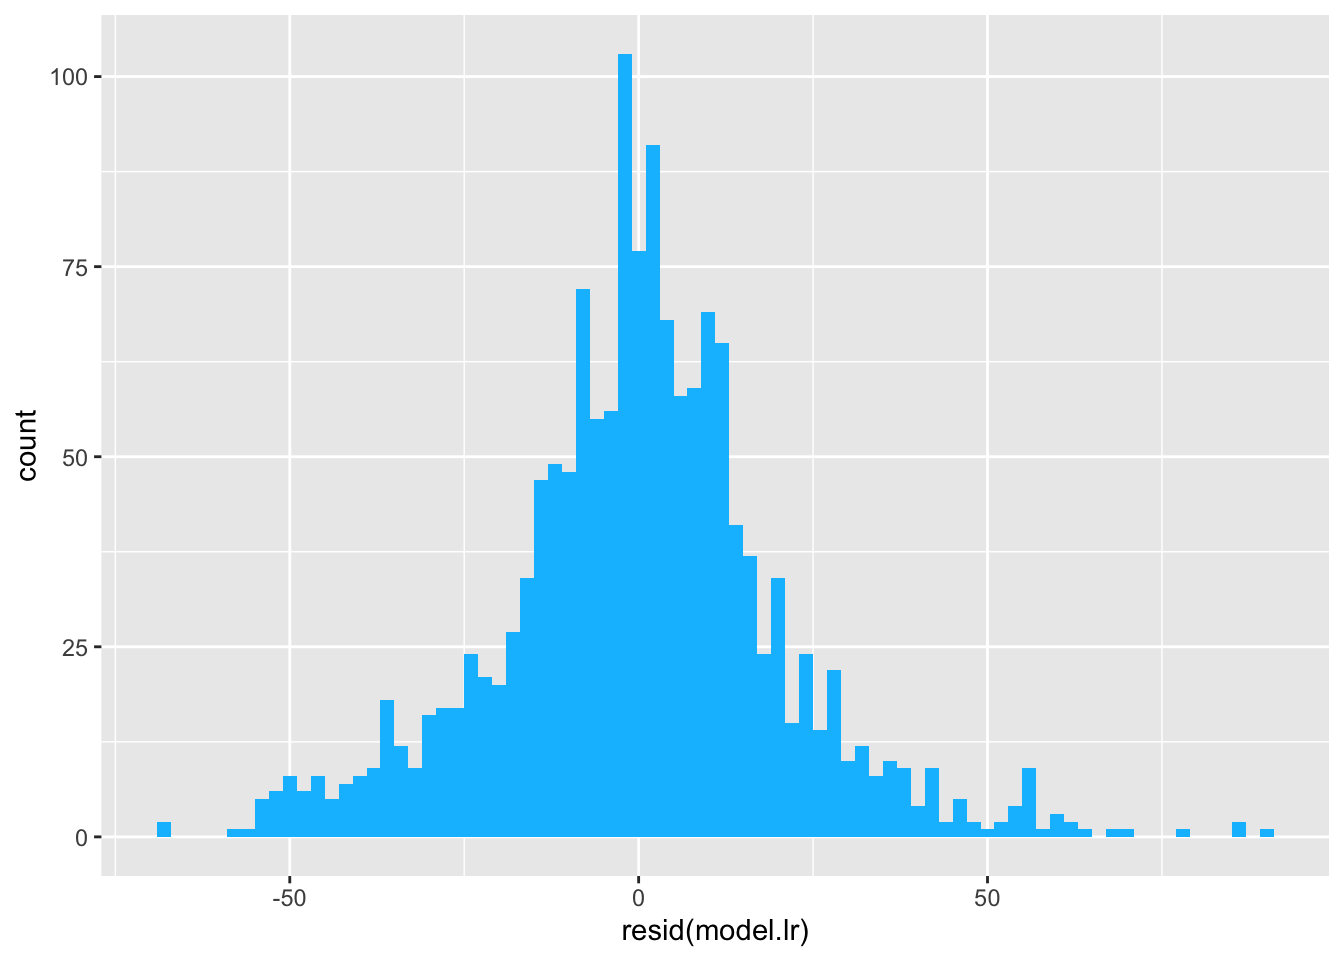
\includegraphics[width=0.8\textwidth]{graphics/linear_mean.png}
    \caption{Histogram of residuals}
    \label{fig:31}
\end{figure}

We can observe that Residuals distribute mainly around the value 0, which is highly indicates that the residuals is scatter mostly around 0 and disperse equally two side of the graph, leading to the fact that the mean is approximately 0. Therefore, this assumption is met.

\textbf{Testing for Residual Errors have Constant Variance:} We can check this assumption using the Scale-Location plot. In this plot we can see the fitted values vs the square root of the standardized residuals. Ideally, we would want to see the residual points equally spread around the red line, which would indicate constant variance.
\begin{code}{R}
plot(model.lr, which = 3)
\end{code}
\begin{figure}[H]
    \centering
    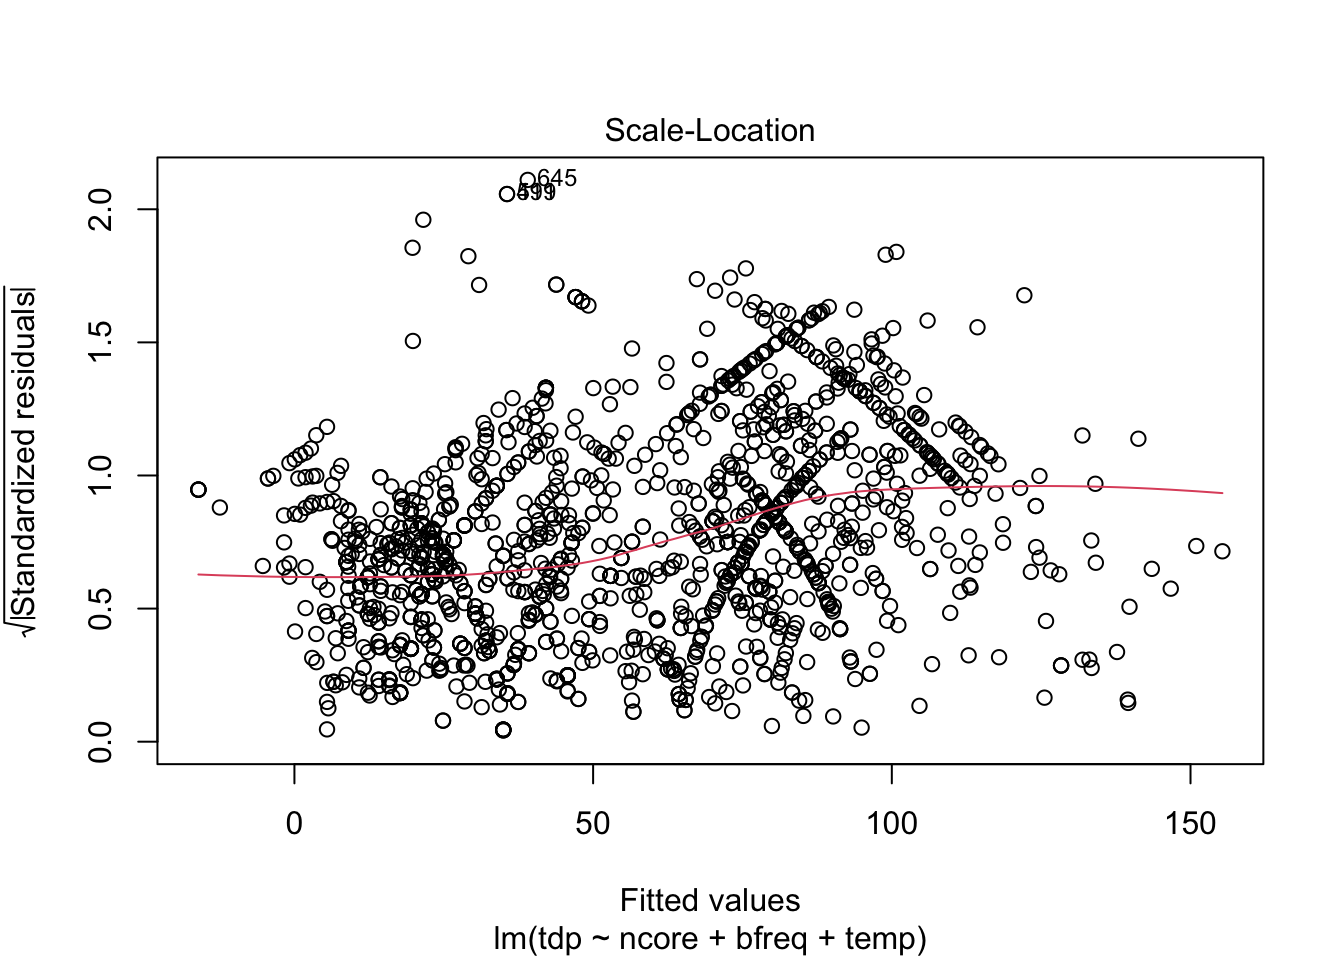
\includegraphics[width=0.8\textwidth]{graphics/linear_scatter.png}
    \caption{Scale-Location plot}
    \label{fig:32}
\end{figure}

In the above plot, we can see that the residual points are equally spread out in a weird pattern, or in other words the residuals scatter is not following any formal distribution and is random. Thus, this assumption is met.

\textbf{Testing for normality of the the errors:} To check this, we have to use Q-Q plot for normality consideration. The output we expect that the residuals will mostly scatter close to the straight line to get normality hypothesis accepted.
\begin{code}{R}
plot(model.lr, which = 2)
\end{code}
\begin{figure}[H]
    \centering
    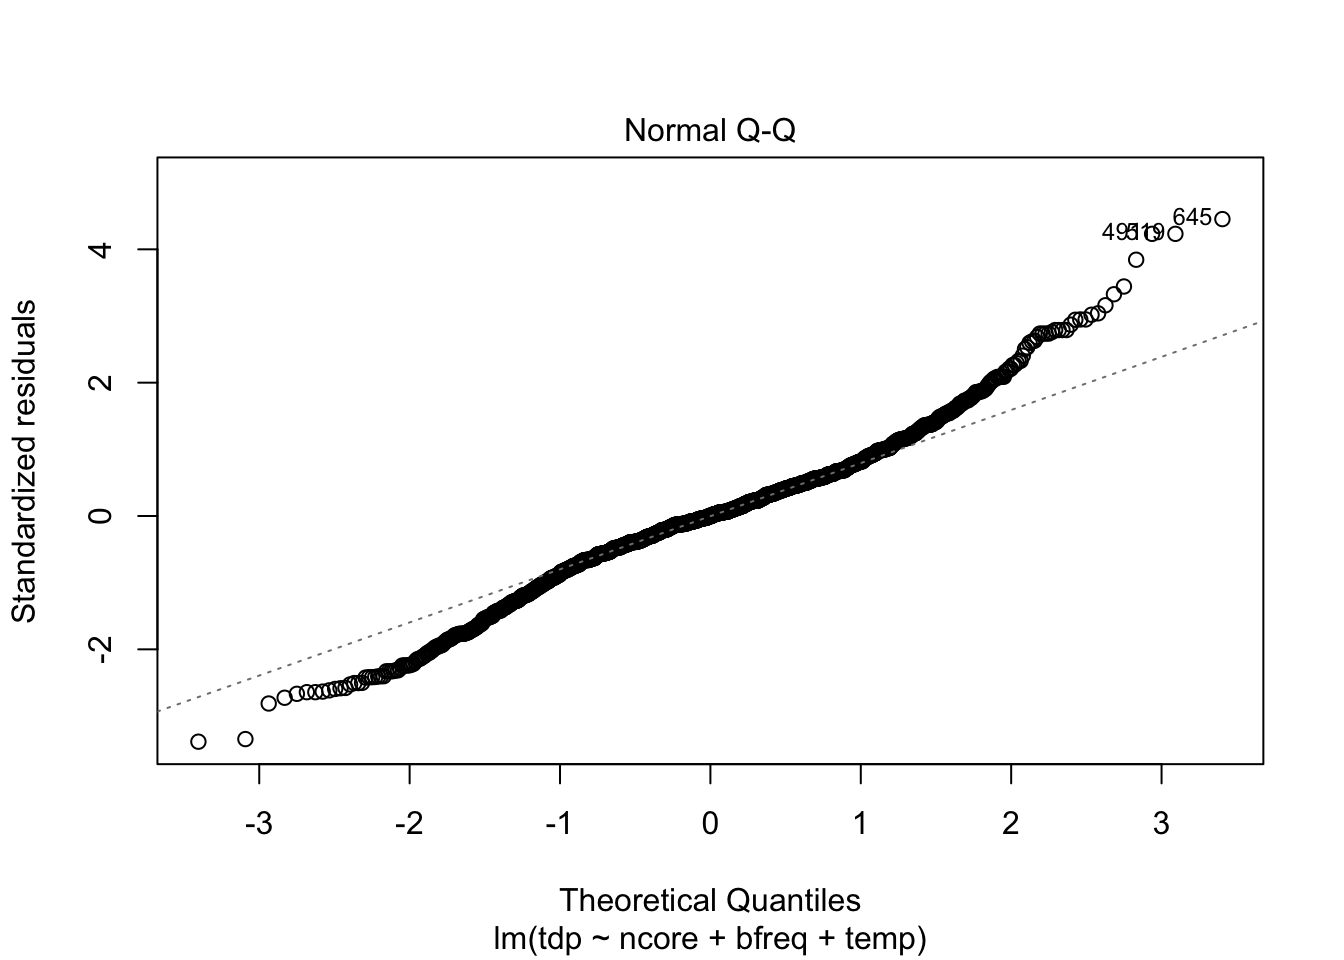
\includegraphics[width=0.8\textwidth]{graphics/linear_normal.png}
    \caption{Q-Q plot for residuals}
    \label{fig:33}
\end{figure}

In the Q-Q plot, it can be seen that those points are lying near the line, while only a few tail points are not lying near the line. We can conclude that this model can be normally accurate, not $100\%$ accurate. Perhaps another model will be more fitted for this data.

When we look at the summary table, the value of multiple $R^2$ is approximately 0.7777, it means that 77.77\% of thermal design power variable is explained by the model and the rest 22.23\% is defined by other factors, which is still accountable but not high. This model so far performing very well.

We will do the scatter plotting for the predicted value of test set compared with real values of the dataset using \verb|plot()| function for more clear vision of this trend.
\begin{code}{R}
# Create data frame for real tdp value and predicted tdp value (for Testing the test set)
comtab.lr <- test['tdp']
comtab.lr['tdp_predicted'] <- as.data.frame(predict(model.lr, newdata = test))
# Plotting
# The majority of points lie near the line, so its ok.
ggplot(comtab.lr, aes(x = tdp, y = tdp_predicted)) +
  geom_point(shape=1, color="blue") +
  geom_abline(mapping=aes(intercept= 0, slope = 1), color="darkblue") +
  labs(x = "TDP", y = "TDP Predicted")
\end{code}
\begin{figure}[H]
    \centering
    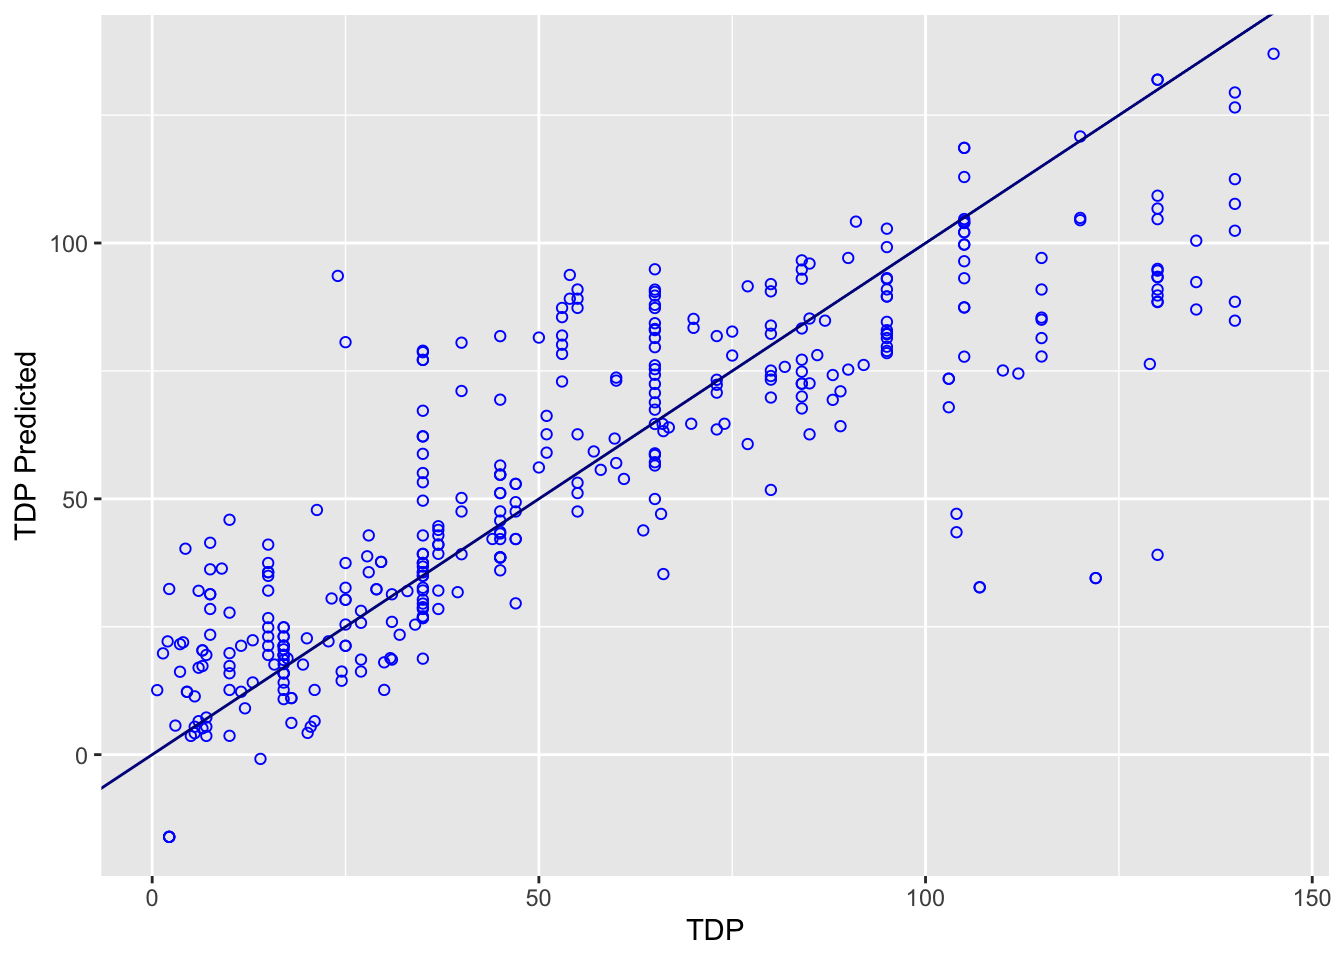
\includegraphics[width=0.8\textwidth]{graphics/linear_predict.png}
    \caption{Predict comparing}
    \label{fig:34}
\end{figure}

At the end of this model, we will do the scatter plotting for the predicted value compared with the real value in test set. The plotted line in graph is $(d): y = x$. The more concentration on this line the more correct the model does.

\textbf{In conclusion}, this model is an acceptable evaluation with the data set, which is shown by the above figures. Nevertheless, the initial assumption about data set's linearity is our subjective point of view, and that is the reason why we continue with the next model.


\subsubsection{Random Forrest Regression Model}
\label{section:data_analysis_randomforrest}
In this section, we will introduce \emph{Random Forest Regression model}. In fact, Random Forest Regression models are often used for predicting system performance metrics such as CPU usage, response time, and throughput. The algorithm can handle both continuous and categorical data, making it a suitable choice for modeling CPU attribute data that may contain a mix of numerical and categorical variables.\\\\
With the second point of view, when we consider the correlation between \verb|TDP| and 3 other ones: number of core, base frequency and temperature, there are many vertical lines created in the scatter-plot graphs. It can be understood as an independence between these variables, simultaneously, the non-linear relationships are also be observed clearly in these graphs.

First, we will build the Random Forest regression model:
\begin{code}{R}
# Build model
model.rfr <- randomForest(formula = tdp ~ bfreq + ncore + temp, data = train, ntree = 500)
# Print model's information
print(model.rfr)
\end{code}

The console the return the summary of the model
\begin{figure}[H]
    \centering
    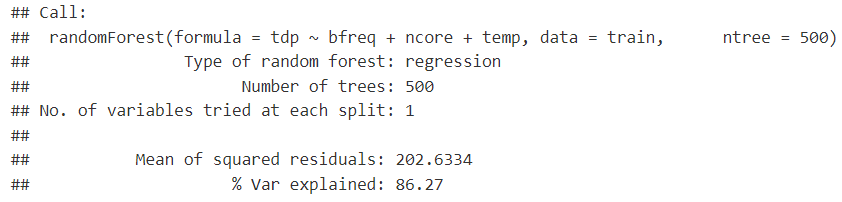
\includegraphics[width = 0.9\textwidth]{graphics/randomSum.png}
    \caption{Random Forest Regression}
    \label{fig:randomForest}
\end{figure}

In the output above, the “$\%$ Var explained” (percentage of variance explained) is a measure of the amount of variation in the target variable that is explained by the random forest regression model. Specifically, it represents the percentage of the total variance in the target variable that is accounted for by the model, and \textit{a higher percentage of variance explained is considered better}, as it indicates that the model is able to explain a larger proportion of the variation in the target variable.

An $\%$ variance explained of $86.27\%$ is generally considered to be a good result for a random forest regression model, as it suggests that the model is able to explain a significant amount of the variation in the target variable.

Another method to test the fitness of this model is checking the \textbf{Mean Absolute Error} (MAE) of this model. The lower the MAE, the better this model validates our hypothesis. To check MAE, using the following commands:
\begin{code}{R}
# Create data frame for real tdp value and predicted tdp value
comtab.rfr <- test['tdp']
comtab.rfr['tdp_predicted'] <- as.data.frame(predict(model.rfr, newdata = test), row.names = NULL)
# Evaluate model performance
accuracy <- sum(1-abs(comtab.rfr$tdp_predicted - comtab.rfr$tdp) / comtab.rfr$tdp) / nrow(comtab.rfr)
MAE <- sum(abs(comtab.rfr$tdp_predicted - comtab.rfr$tdp)) / nrow(comtab.rfr)
print(paste("Accuracy:", accuracy))
print(paste("MAE:", MAE))
\end{code}

This yields the output in the console
\begin{figure}[H]
    \centering
    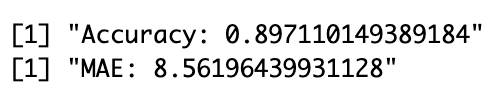
\includegraphics[width=0.45\textwidth]{graphics/MAE.png}
    \caption{Mean Absolute Error}
    \label{fig:MAE}
\end{figure}
The MAE represents the average absolute difference between the predicted and actual values of the target variable, across all observations in the data set. It is calculated by taking the mean of the absolute values of the differences between the predicted and actual values taken from the \textbf{test set} we divided before.

The acceptable level of MAE depends on the specific problem and the context in which the model is being used. In general, a lower MAE is considered better, as it indicates that the model is making more accurate predictions. In this case, the error MAE value is $8.56196$ which is relatively small compare to the range of the data, moreover, the accuracy of this model is approximately $89.711\%$, which is very high, indicating that this model is reliable. Similarly with the R-squared validation, to compute the R-squared value, we use the following commands:
\begin{code}{R}
# calculate R-squared on testing data
r2_test <- cor(comtab.rfr$tdp, comtab.rfr$tdp_predicted)^2
print(r2_test)
\end{code}

The output in the console is
\begin{figure}[H]
    \centering
    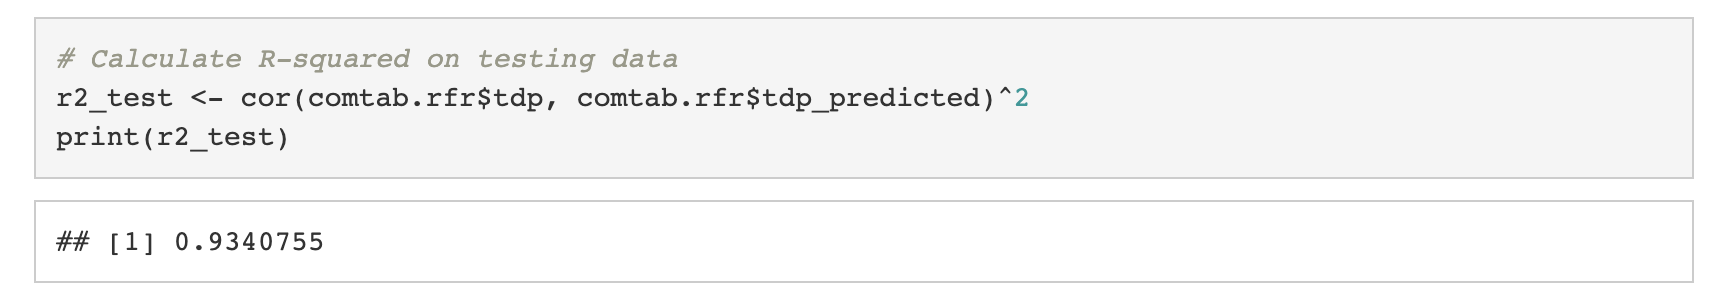
\includegraphics[width=0.9\textwidth]{graphics/RsquaredRandom.png}
    \caption{R-squared Value}
    \label{fig:RSV}
\end{figure}

Similarly in the previous model, the closer the value R-squared to 1, the more fitted the model is, which in this case is 0.9340755 very close to 1 so this strengthen the alternative hypothesis that there is a significant relationship between these features.

Because the assumption of this Random Forest model requires that the residual must follow normal distribution, we will use Q-Q plot to test if the residuals is normally distributed:
\begin{code}{R}
# Calculate the residuals by subtracting the actual values from the predicted values
residuals <- comtab.rfr$tdp - comtab.rfr$tdp_predicted

# Create a normal probability plot of the residuals
qqnorm(residuals)
qqline(residuals)
\end{code}
\begin{figure}[H]
    \centering
    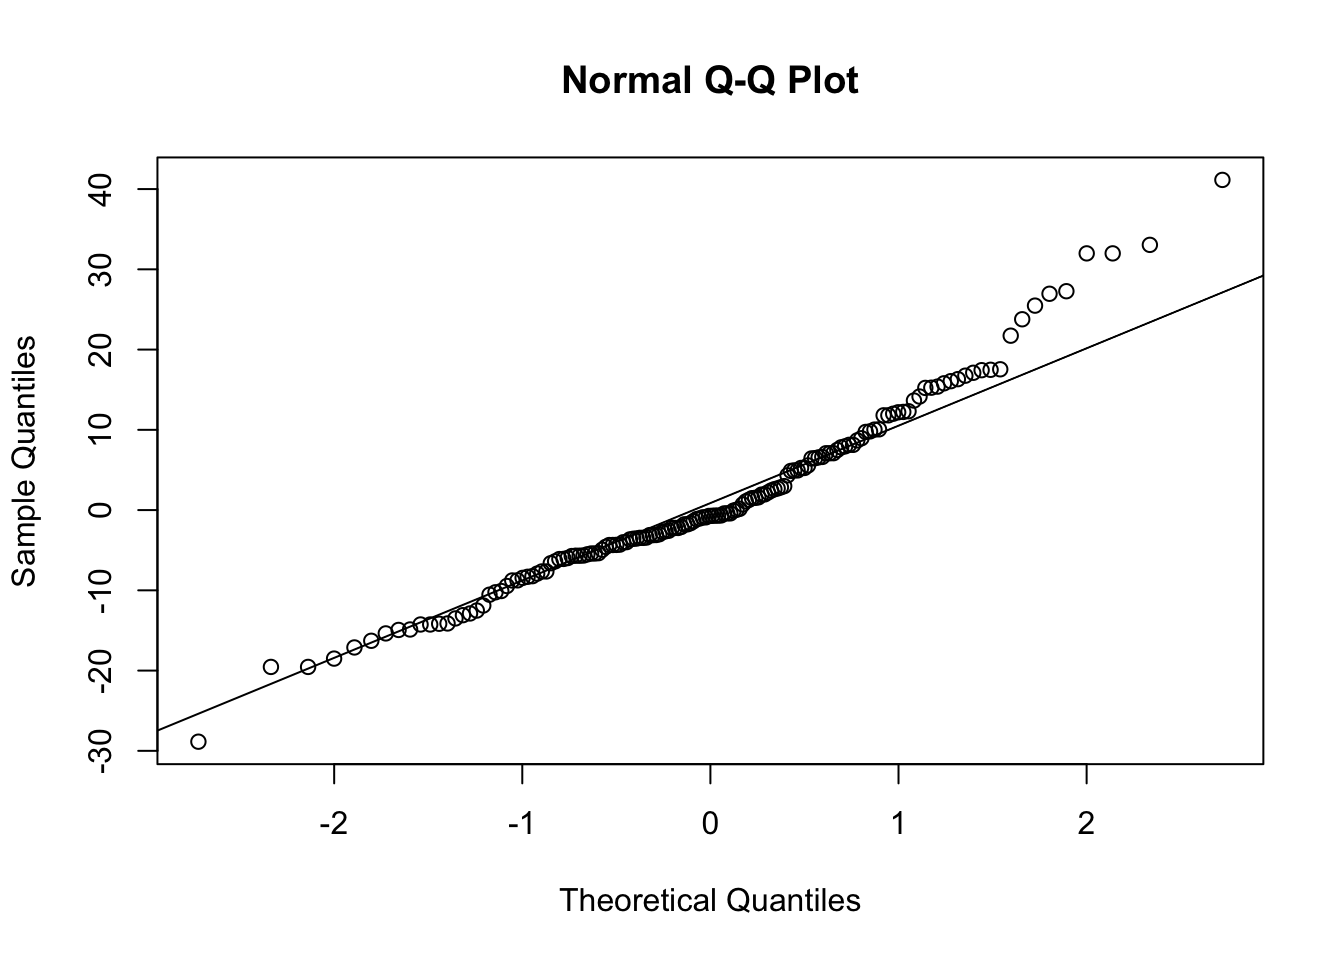
\includegraphics[width=0.9\textwidth]{graphics/randomQQplot.png}
    \caption{Theoretical quantiles Plot}
    \label{fig:QQ}
\end{figure}

In the Q-Q plot, it can be seen that those points are not fully lying near the line. We can conclude that this model may not be normally accurate.\\

We will do the scatter plotting for the predicted value of test set compared with real values of the \textbf{test} data set using \verb|plot()| function:
\begin{code}{R}
# Plot the predicted - actual
ggplot(comtab.rfr, aes(x = tdp, y = tdp_predicted)) +
  geom_point(shape = 1, color = "blue") +
  geom_abline(mapping = aes(intercept = 0, slope = 1), color = "darkblue") +
  labs(x = "TDP", y = "TDP Predicted")
\end{code}
\begin{figure}[H]
    \centering
    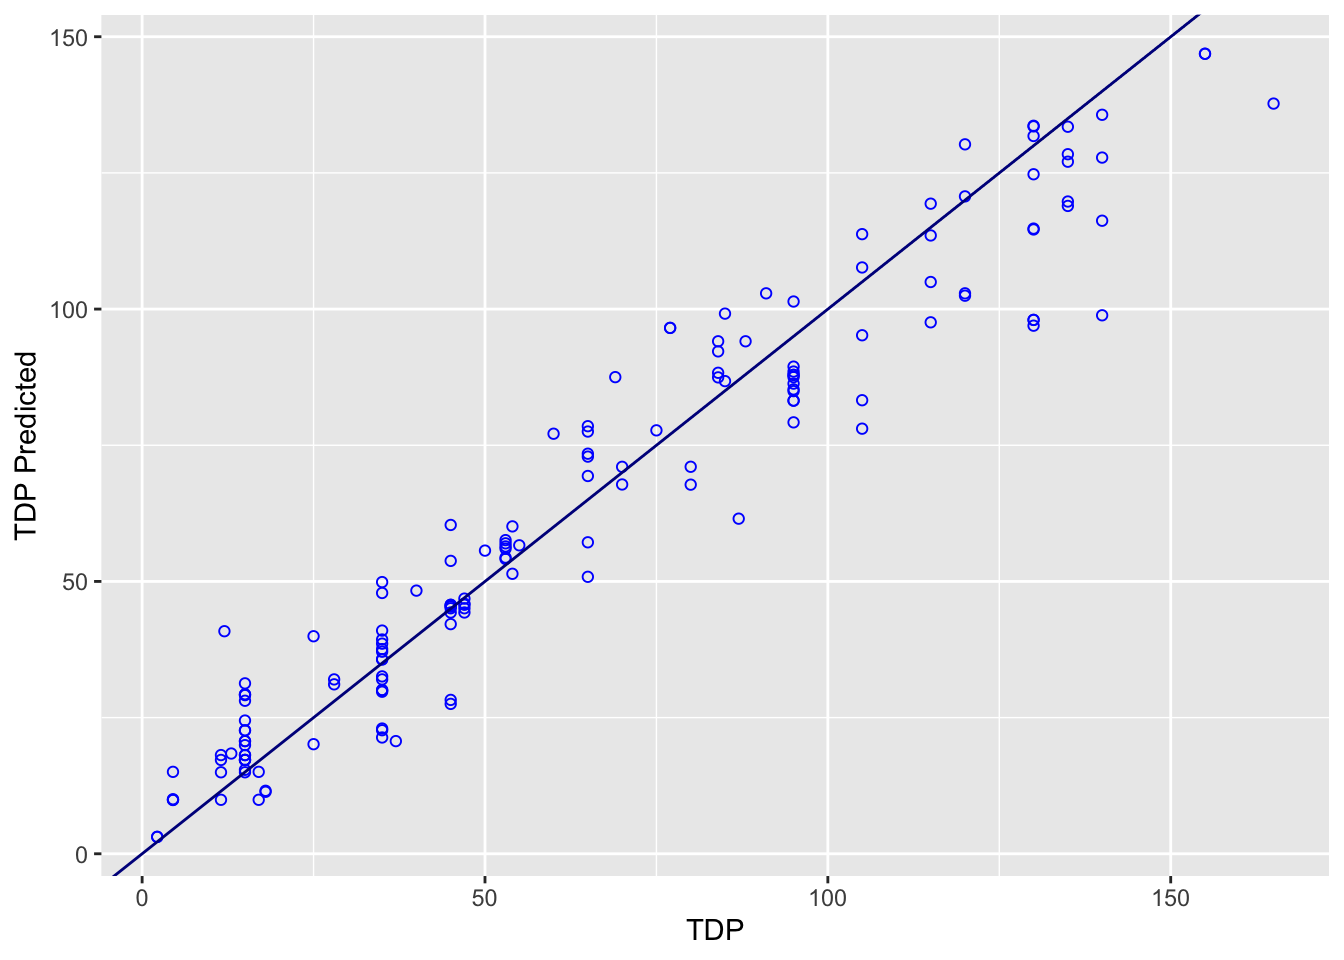
\includegraphics[width=0.7\textwidth]{graphics/randomPlot.png}
    \caption{Random Forest model prediction}
    \label{fig:random_trend}
\end{figure}

As we can see, the closer the points to the line, the more accurate the prediction, and we clearly see, similarly to the previous model, this is somewhat like $80\%$ normally distributed in residuals, which is explained most of the variables involved.

\textbf{In conclusion}, compared to Linear regression model, the current model - Random forest give us the more optimistic results which are proven in the above figures such as error, accuracy and \(R^2\) value. As a result, we conclude this model is fitter to our data and get the quite high results, not 100\% accuracy. Perhaps, more data should be obtained or some indexes such as number of tree be modified to reach the higher accuracy.














%
%   Conclusion
%
%   What did we find?
%   
\clearpage
\section{Conclusion}
In general, we have conducted several test models and received many positive outcomes that provide strong proof to reject the null hypothesis that there is no significant relationship between these categories, therefore confirming our prediction that the thermal power design of each CPU strongly depends on the number of cores and base frequency, as well as the temperature that can occur when entering hard mode of task of the devices it is attached on, leaving chip producer a clearer view to balance out between the power consumption and the performance of the chips to better their benefits in the technology field.

With the topic \textbf{Researching on the Thermal Design Power of CPU} uses the R programming language to process statistical data and realize the model linear regression model, our team had a more intuitive view of how to extract data, process and analyze raw data, turning them into valuable data sources long-term, or better yet, being able to generalize the general situation and make predictions about the data set.

During the process of implementing the thesis will not be able to avoid some minor errors, as well as some of the predictions might not be exactly as reality, our group hopes that this thesis report will provide another aspect for the viewers about the issue of dealing with the Thermal Design Power problem in the real world.



\bibliographystyle{plainnat}
\bibliography{refs.bib}
\addbibresource{refs.bib}
\nocite{*}
\end{document}